\documentclass{article}

\usepackage{lipsum}
\usepackage{amsfonts}
\usepackage{amsmath}
\usepackage{amsthm}
\usepackage{graphicx}
\graphicspath{{figures/1_27_22/}}
\usepackage{epstopdf}
\ifpdf%
\DeclareGraphicsExtensions{.eps,.pdf,.png,.jpg}
\else
\DeclareGraphicsExtensions{.eps}
\fi
\usepackage{amsopn}
\DeclareMathOperator{\diag}{diag}
\usepackage{booktabs}
\usepackage{bbm}
\usepackage{bm}
\usepackage{caption}
\usepackage{subcaption}
\usepackage[utf8]{inputenc}
\usepackage[T1]{fontenc}
\usepackage[margin=1in]{geometry}
\usepackage{hyperref}
\usepackage{algorithm}
\usepackage{algpseudocode}

\newcommand{\norm}[1]{\left\lVert#1\right\rVert}
\newcommand{\normtwo}[1]{\left\lVert#1\right\rVert_2}
\newcommand{\abs}[1]{\left\lvert#1\right\rvert}
\newcommand{\mat}[1]{\bm{{#1}}}
\renewcommand{\vec}[1]{\bm{{#1}}}
\newcommand{\lequiv}{\Leftrightarrow}
\newcommand{\bigO}[1]{\mathcal{O}\!\left(#1\right)}
\newcommand{\ceil}[1]{\left\lceil #1 \right\rceil}
\newcommand{\floor}[1]{\left\lfloor #1 \right\rfloor}
\newcommand{\sfrac}[2]{#1/#2}
\newcommand{\hquad}{\enskip}
\newcommand{\expected}[1]{\mathbb{E}\left[#1\right]}
\newcommand{\mspan}[1]{\text{span}\left( #1 \right)}
\newcommand{\prob}[1]{P\left(#1\right)}
\newcommand{\probt}[1]{P\left( \text{#1} \right)}
\newcommand{\condprob}[2]{P\left(#1 \:|\: #2\right)}
\newcommand{\condprobt}[2]{P\left(\text{#1} \:|\: \text{#2}\right)}
\newcommand{\bayes}[2]{\frac{\condprob{#2}{#1}\prob{#1}}{\prob{#2}}}
\newcommand{\bayesx}[3]{\frac{\condprob{#2}{#1}\prob{#1}}{\condprob{#2}{#1}\prob{#1} + \condprob{#2}{#3}\prob{#3}}}
\newcommand{\sech}{\text{sech}}
\newcommand*{\vertbar}{\rule[-1ex]{0.5pt}{2.5ex}}
\newcommand*{\horzbar}{\rule[.5ex]{2.5ex}{0.5pt}}
\newcommand{\vect}[2]{\underline{{#1}}_{{#2}}}
\newcommand{\basisp}[1]{\underline{{p}}_{{#1}}}
\newcommand{\basisq}[1]{\underline{{q}}_{{#1}}}
\newcommand{\coeff}[1]{\underline{{a}}_{{#1}}}
\newcommand{\bestfit}{\underline{\bar{x}}}
\newcommand{\grad}{\nabla}
\newcommand{\laplace}{\Delta}
\newcommand{\setbar}{\:\middle|\:}
\renewcommand{\div}{\grad \cdot}
\renewcommand{\Re}{\text{Re}}

\begin{document}
\section{Background}
Here, we are attempting to train an ML agent to output both aggregates and interpolation for an AMG solver given some matrix $\mat{A}$.  We will explore how well such an agent can learn to generalize on an \textit{isotropic diffusion problem}, by generating datasets of \textit{only unstructured problems}:
\begin{enumerate}
\item A training set of 1000 unstructured grids
\item A testing set of 250 unstructured grids
\end{enumerate}
Each of these grid meshes are fairly small, overall containing between around 15 and 400 points.  To create a mesh, random points are generated in $\left[0,1\right]^2$, a convex hull constructed, then meshed with gmsh.  However, due to computational costs, only $1/4$ of the training and testing sets are loaded to reduce overall training time.

\section{Generating Aggregates and Interpolation}
To compute the aggregates and final interpolation operator, two individual networks are trained concurrently to perform each action, which we will label $\Theta_{\text{Agg}}$ and $\Theta_{\text{Interp}}$, both taking some weighted graph and returning a new graph with same connectivity, but different weight values.  The algorithm for finding the aggregates and interpolation is roughly sketched below:
\begin{enumerate}
\item Let $\mat{A} \in \mathbb{R}^{n \times n}$ be the system we are trying to solve and $\alpha \in \left(0, 1\right]$ be some parameter that determines the ratio of aggregates to vertices, i.e. we will be roughly coarsening the graph by $1/\alpha$.  Define $k := \ceil{\alpha n}$, the number of aggregates we will be outputting.
\item Convolve the graph of $\mat{A}$ with $\Theta_{\text{Agg}}$ to obtain a new set of node values, restarting halfway through and inserting the tenative cluster centers as a node feature.  We will use the output node values as a \textit{scoring} and discard any convoled edge values.  Define the aggregate centers as the indices of the largest $k$ node scores.  Then, run Bellman-Ford on the graph with these aggregate centers to obtain a tentative aggregation operator, $\text{Agg}$.
\item Now, again convolve the graph of $\mat{A}$ but with $\Theta_{\text{Interp}}$ (with aggregate information) to obtain the aggregate smoother $\mat{\hat{P}}$.  Form $\mat{P} := \mat{\hat{P}}\text{Agg}$.
\end{enumerate}

\section{Genetic Training}
Training of both networks is done at the same time with a custom-written genetic algorithm that takes advantage of the easily parallelizable fitness calculation.  A genetic algorithm is used because it does not require any gradient information, which benefits us because the algorithm used to output the aggregates is not easily differentiable.

A basic overview of the training algorithm is that the method is seeded with some number of randomly generated networks. A subset of the best performing (most fit) networks are selected and \textit{bred} with one another (crossing weights/traits) and \textit{mutations} inserted (random perturbations to weights) to create another population of networks.  This is then repeated for many \textit{generations} until a set of hopefully trained networks is obtained, from which we can pick the best fit as our final network.

\begin{figure}[h]
  \centering
  \begin{subfigure}[t]{0.49\textwidth}
    \centering
    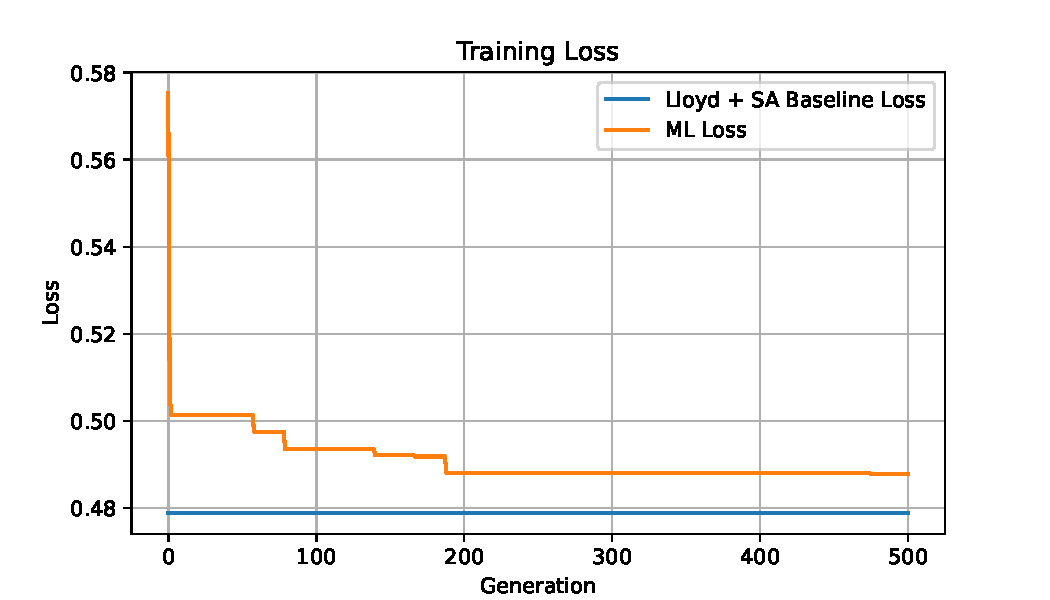
\includegraphics[width=\textwidth]{train_loss.pdf}
    \caption{Training loss}
  \end{subfigure}
  \hfill
  \begin{subfigure}[t]{0.49\textwidth}
    \centering
    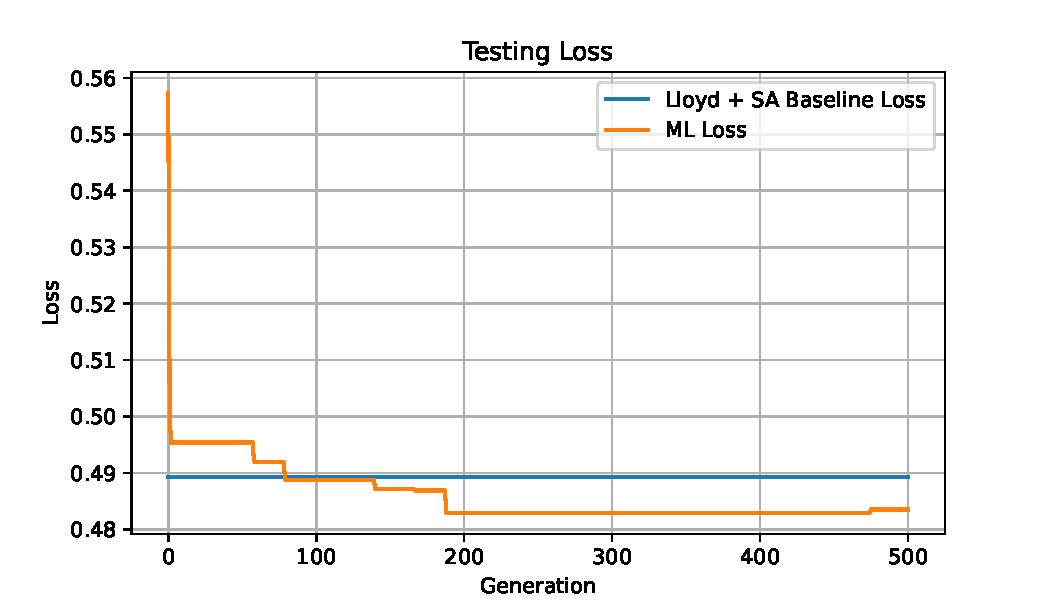
\includegraphics[width=\textwidth]{test_loss.pdf}
    \caption{Testing loss}
  \end{subfigure}
  \caption{Loss plots per generation for training and testing datasets, respectively.}
  \label{fig:loss}
\end{figure}

\begin{figure}[h]
  \centering
  \begin{subfigure}[t]{0.49\textwidth}
    \centering
    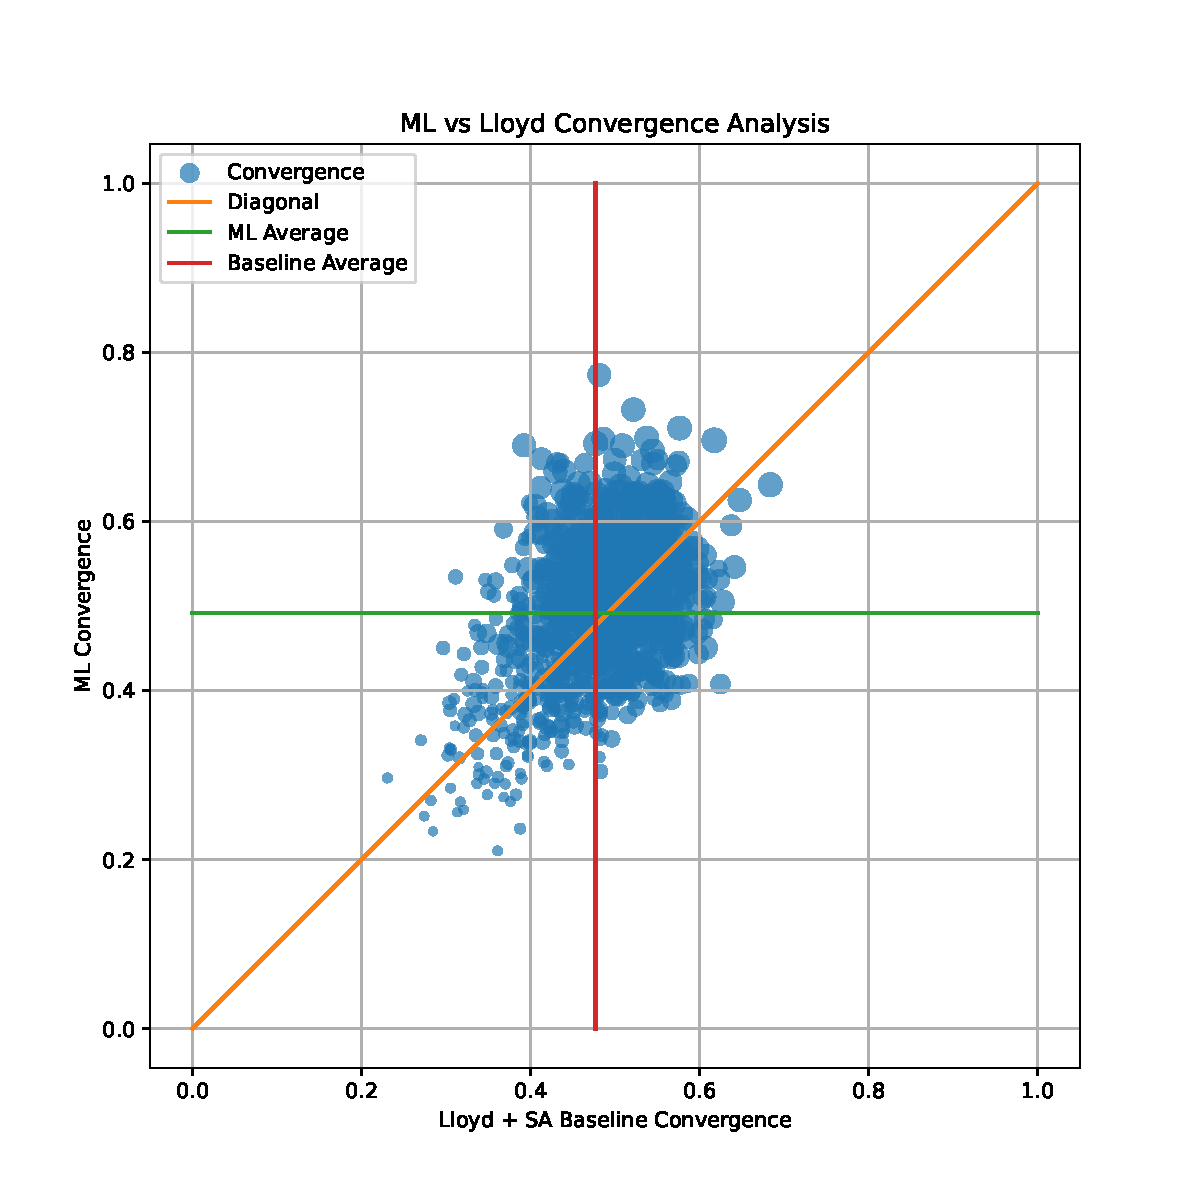
\includegraphics[width=\textwidth]{train_convergence.pdf}
    \caption{Training convergence}
  \end{subfigure}
  \begin{subfigure}[t]{0.49\textwidth}
    \centering
    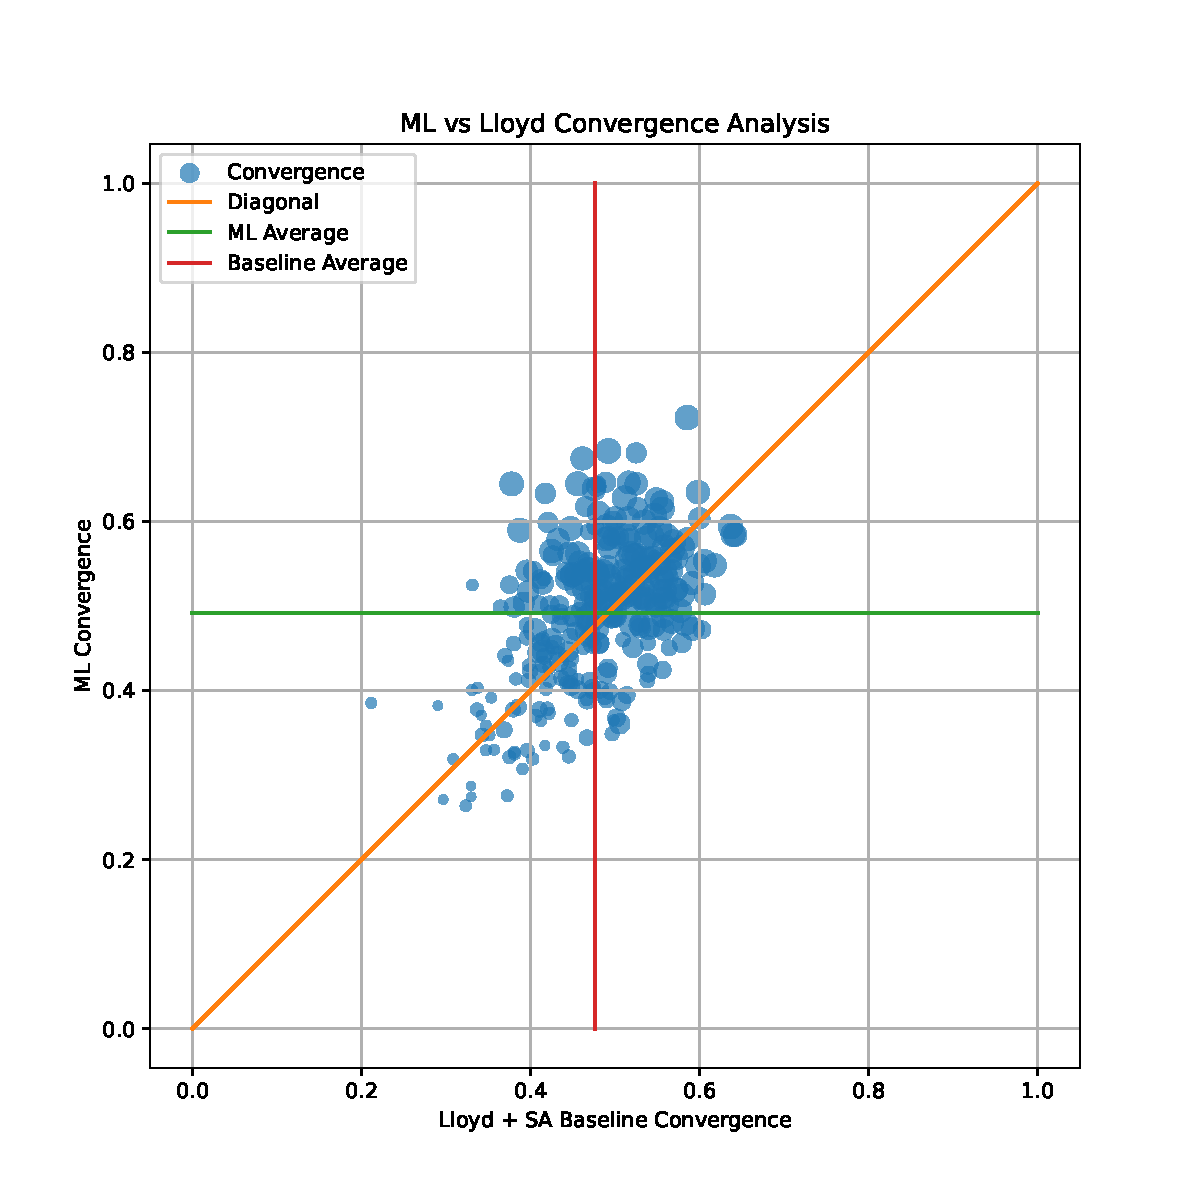
\includegraphics[width=\textwidth]{test_convergence.pdf}
    \caption{Testing convergence}
  \end{subfigure}
  \caption{Convergence data for the ML AMG method vs a baseline Lloyd and Jacobi SA method.  Values below the diagonal indicate a better convergence for the ML.  Markers are scaled by problem size.}
  \label{fig:conv}
\end{figure}

\begin{figure}[h]
  \centering
  \begin{subfigure}[t]{0.49\textwidth}
    \centering
    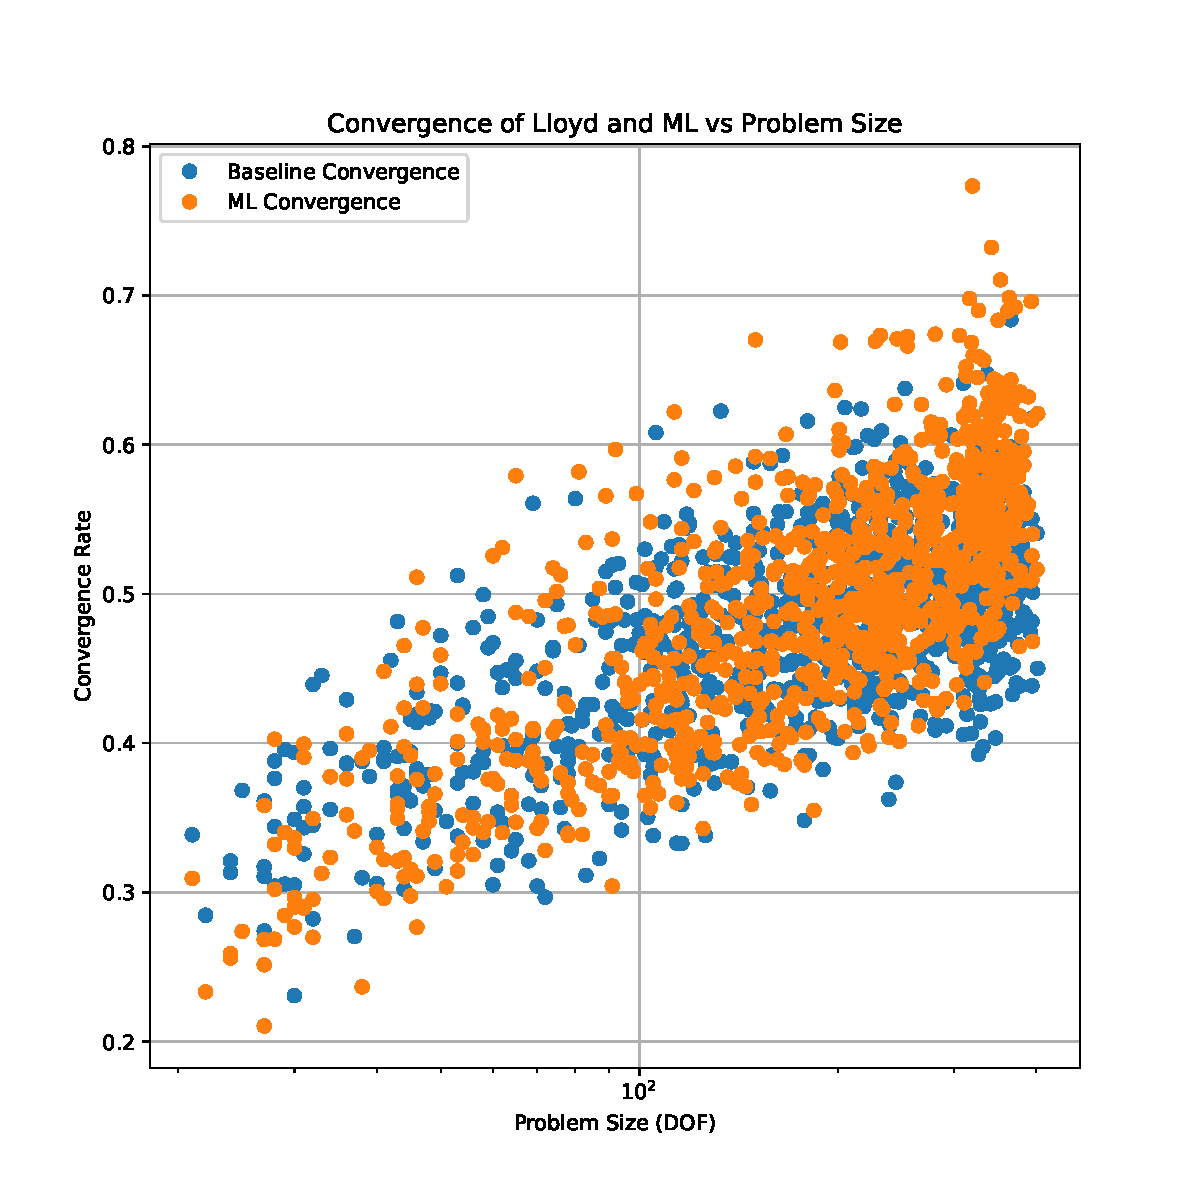
\includegraphics[width=\textwidth]{train_convergence_per_size.pdf}
    \caption{Training convergence}
  \end{subfigure}
  \begin{subfigure}[t]{0.49\textwidth}
    \centering
    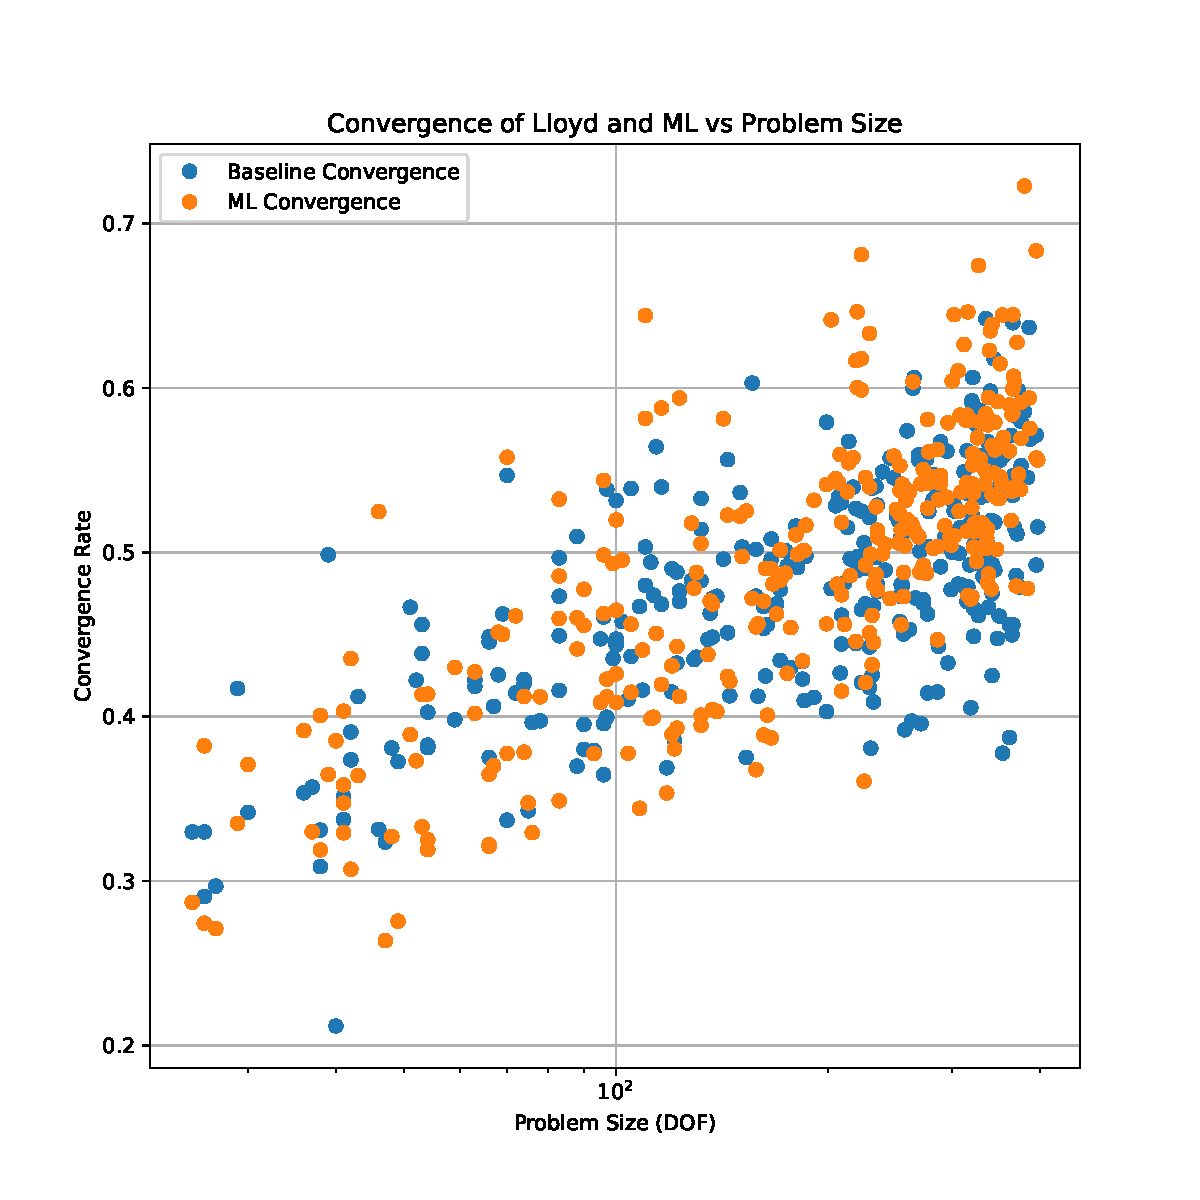
\includegraphics[width=\textwidth]{test_convergence_per_size.pdf}
    \caption{Testing convergence}
  \end{subfigure}
  \caption{Convergence data for the two methods plotted against problem size (DOF).  The ML method seems biased towards better performance on the smaller problems, and does not do as well on the larger problems.}
  \label{fig:conv_per_size}
\end{figure}

\begin{figure}[h]
  \centering
  \begin{subfigure}[t]{0.49\textwidth}
    \centering
    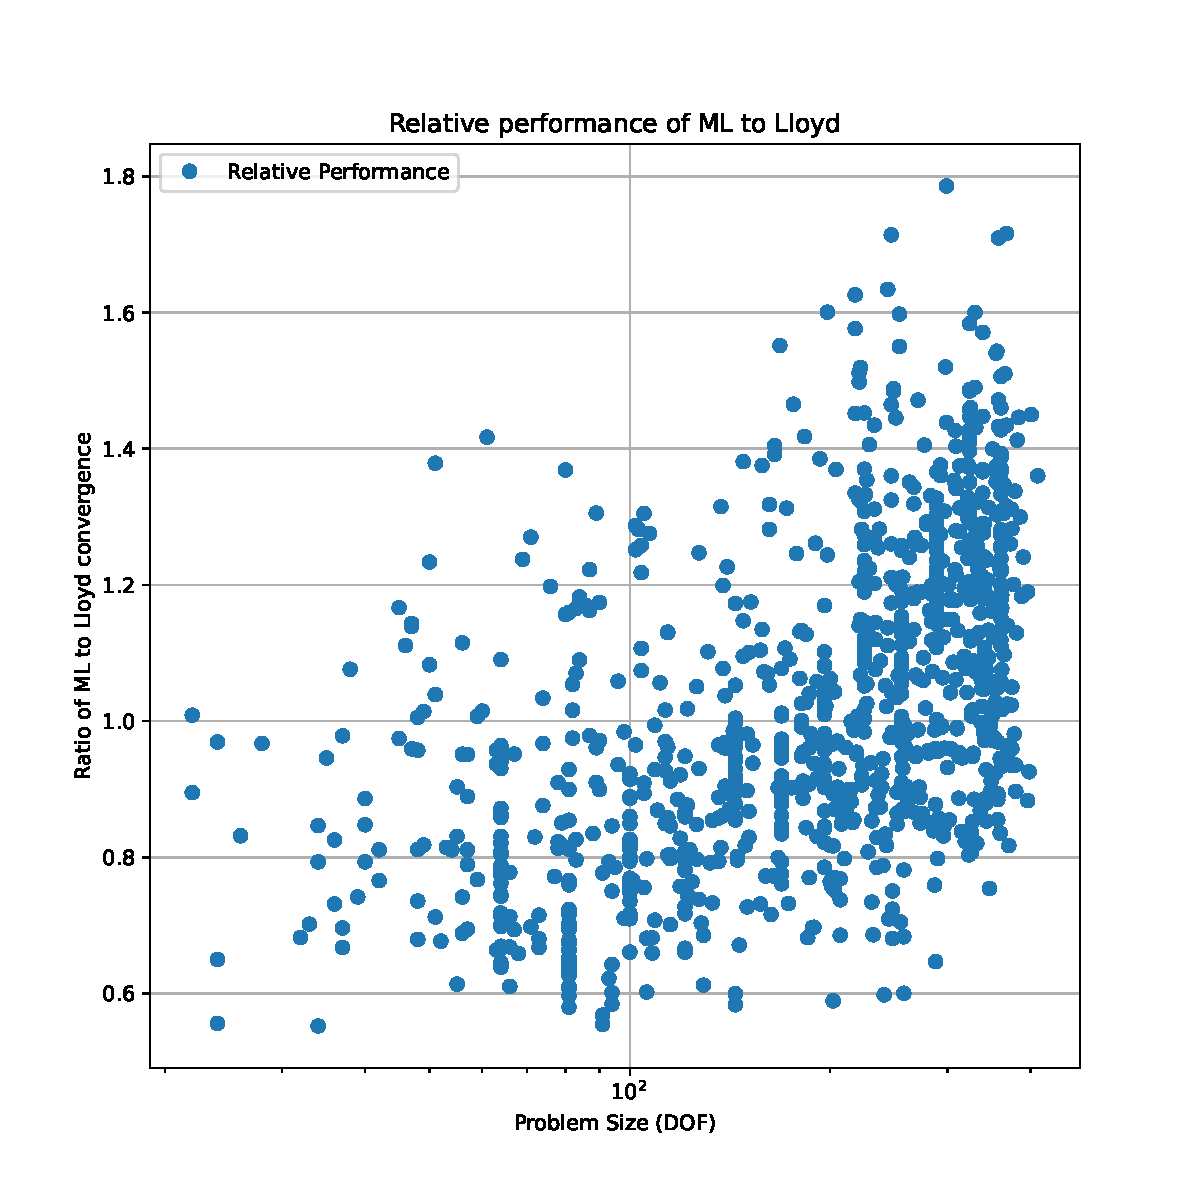
\includegraphics[width=\textwidth]{rel_perf_train.pdf}
    \caption{Relative training performance}
  \end{subfigure}
  \begin{subfigure}[t]{0.49\textwidth}
    \centering
    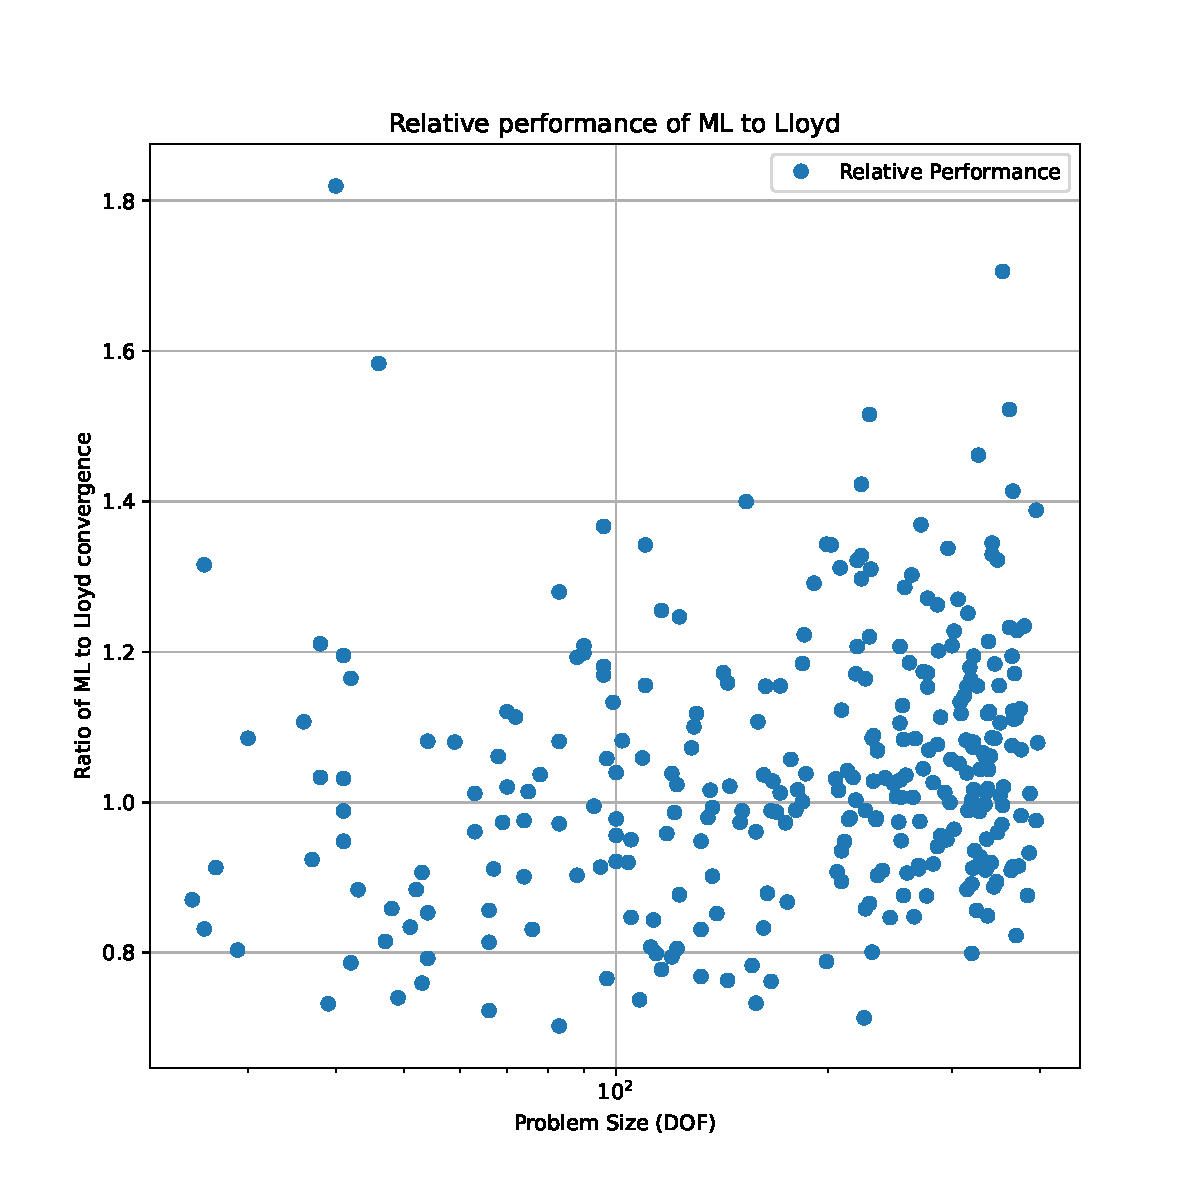
\includegraphics[width=\textwidth]{rel_perf_test.pdf}
    \caption{Relative testing performance}
  \end{subfigure}
  \caption{Relative performance of the ML to the Lloyd method, plotted against problem size.  Relative performance is obtained by dividing the ML convergence by the Lloyd convergence for each problem.}
  \label{fig:rel_conv}
\end{figure}

\begin{figure}[h]
  \centering
  \begin{subfigure}[t]{0.32\textwidth}
    \centering
    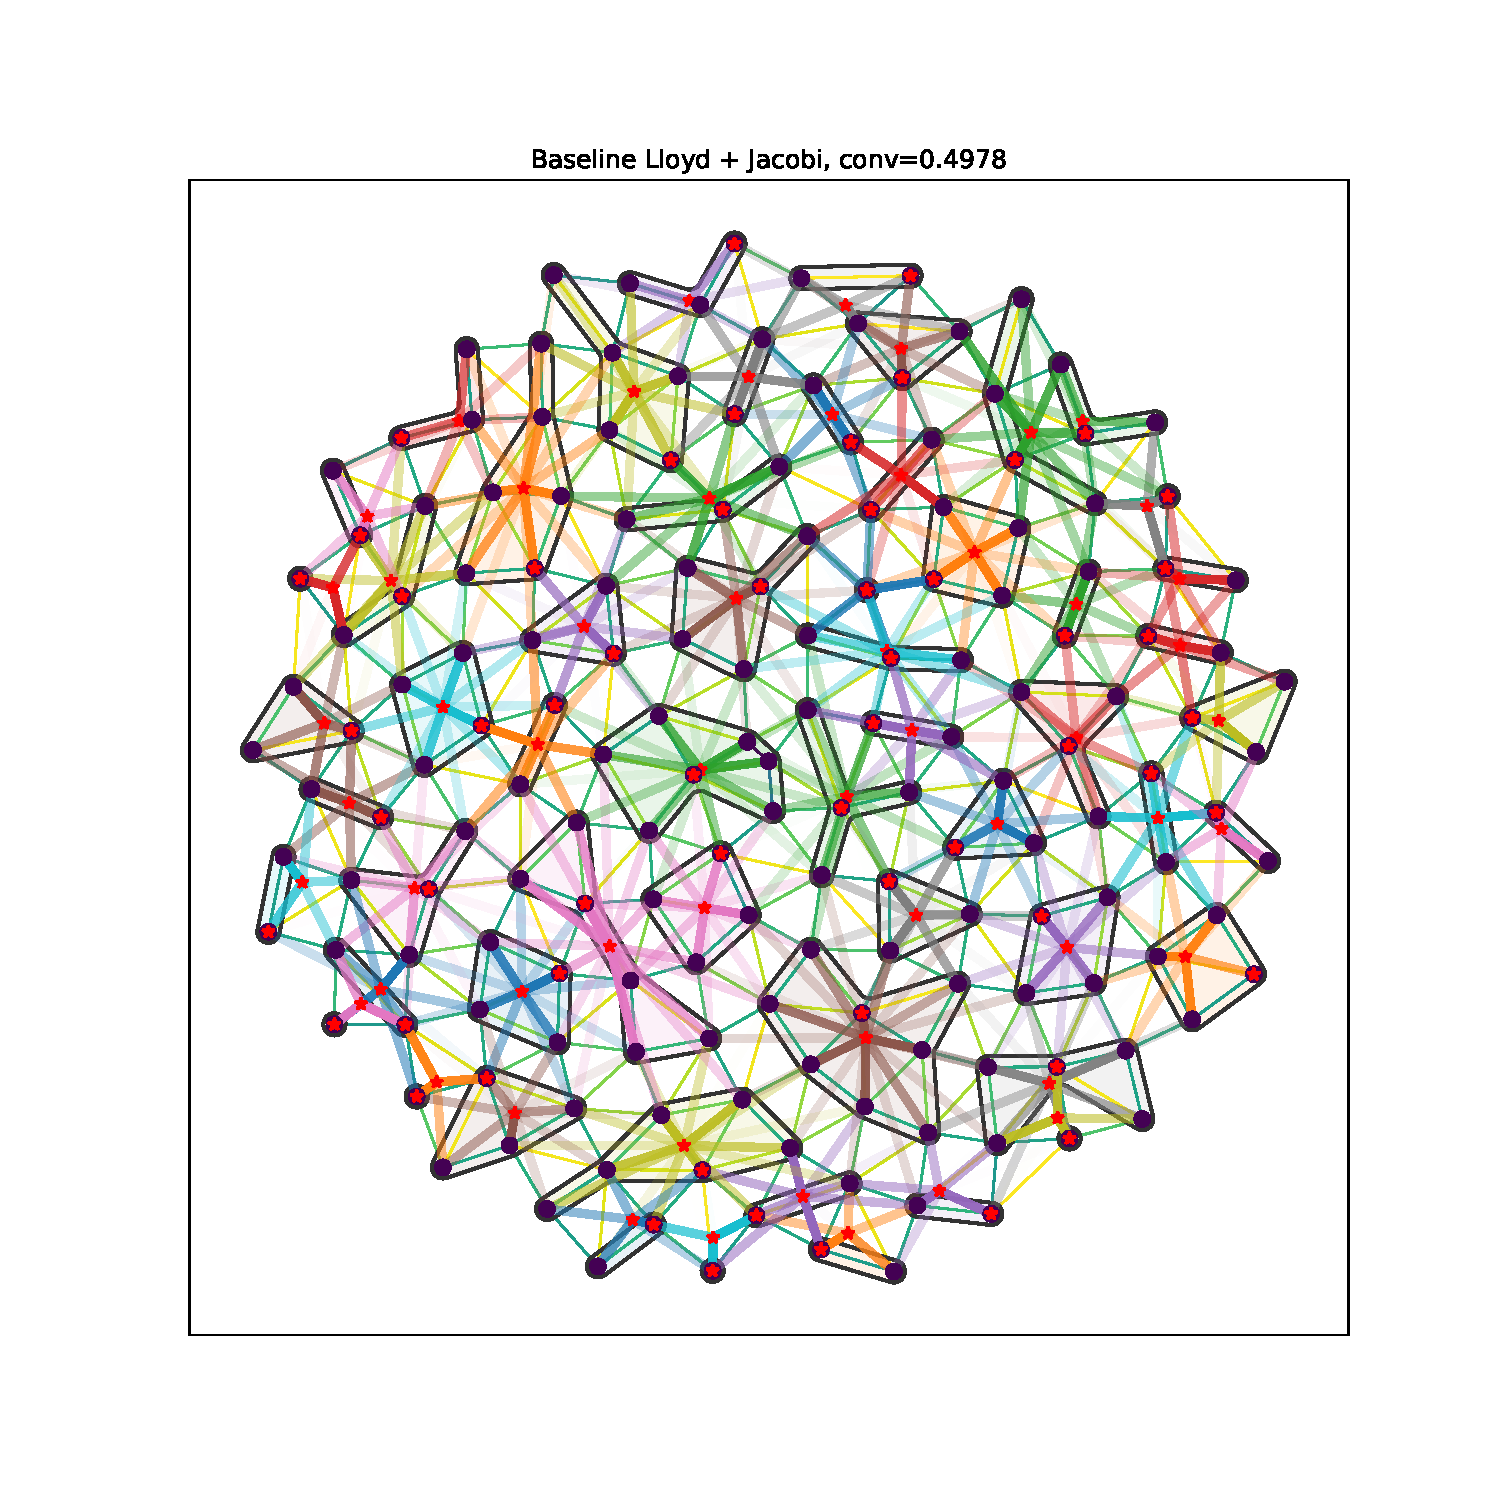
\includegraphics[width=\textwidth, trim=80 70 70 50, clip]{grid_circle_lloyd.pdf}
    \caption{Lloyd + Jacobi}
  \end{subfigure}
  \begin{subfigure}[t]{0.32\textwidth}
    \centering
    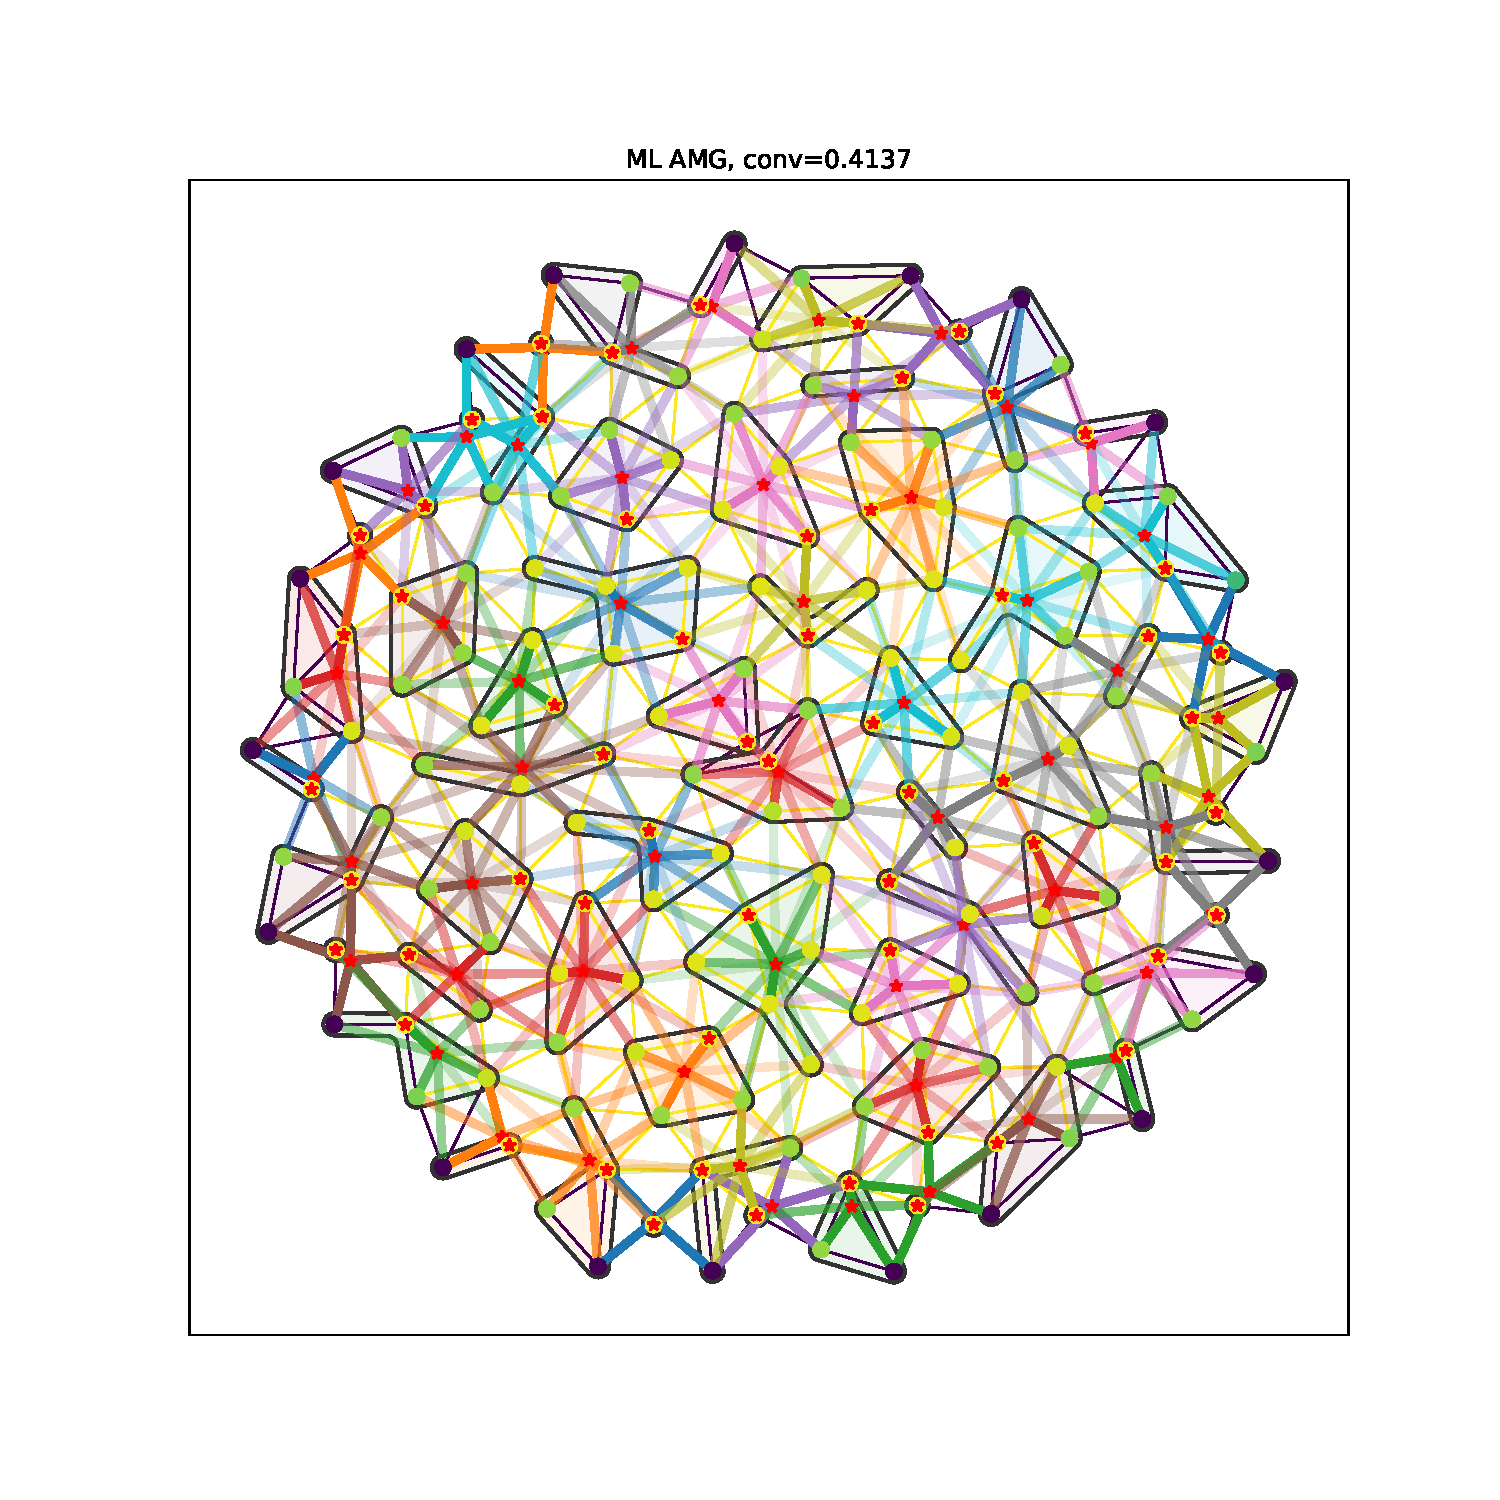
\includegraphics[width=\textwidth, trim=80 70 70 50, clip]{grid_circle_ml.pdf}
    \caption{ML}
  \end{subfigure}
  \begin{subfigure}[t]{0.32\textwidth}
    \centering
    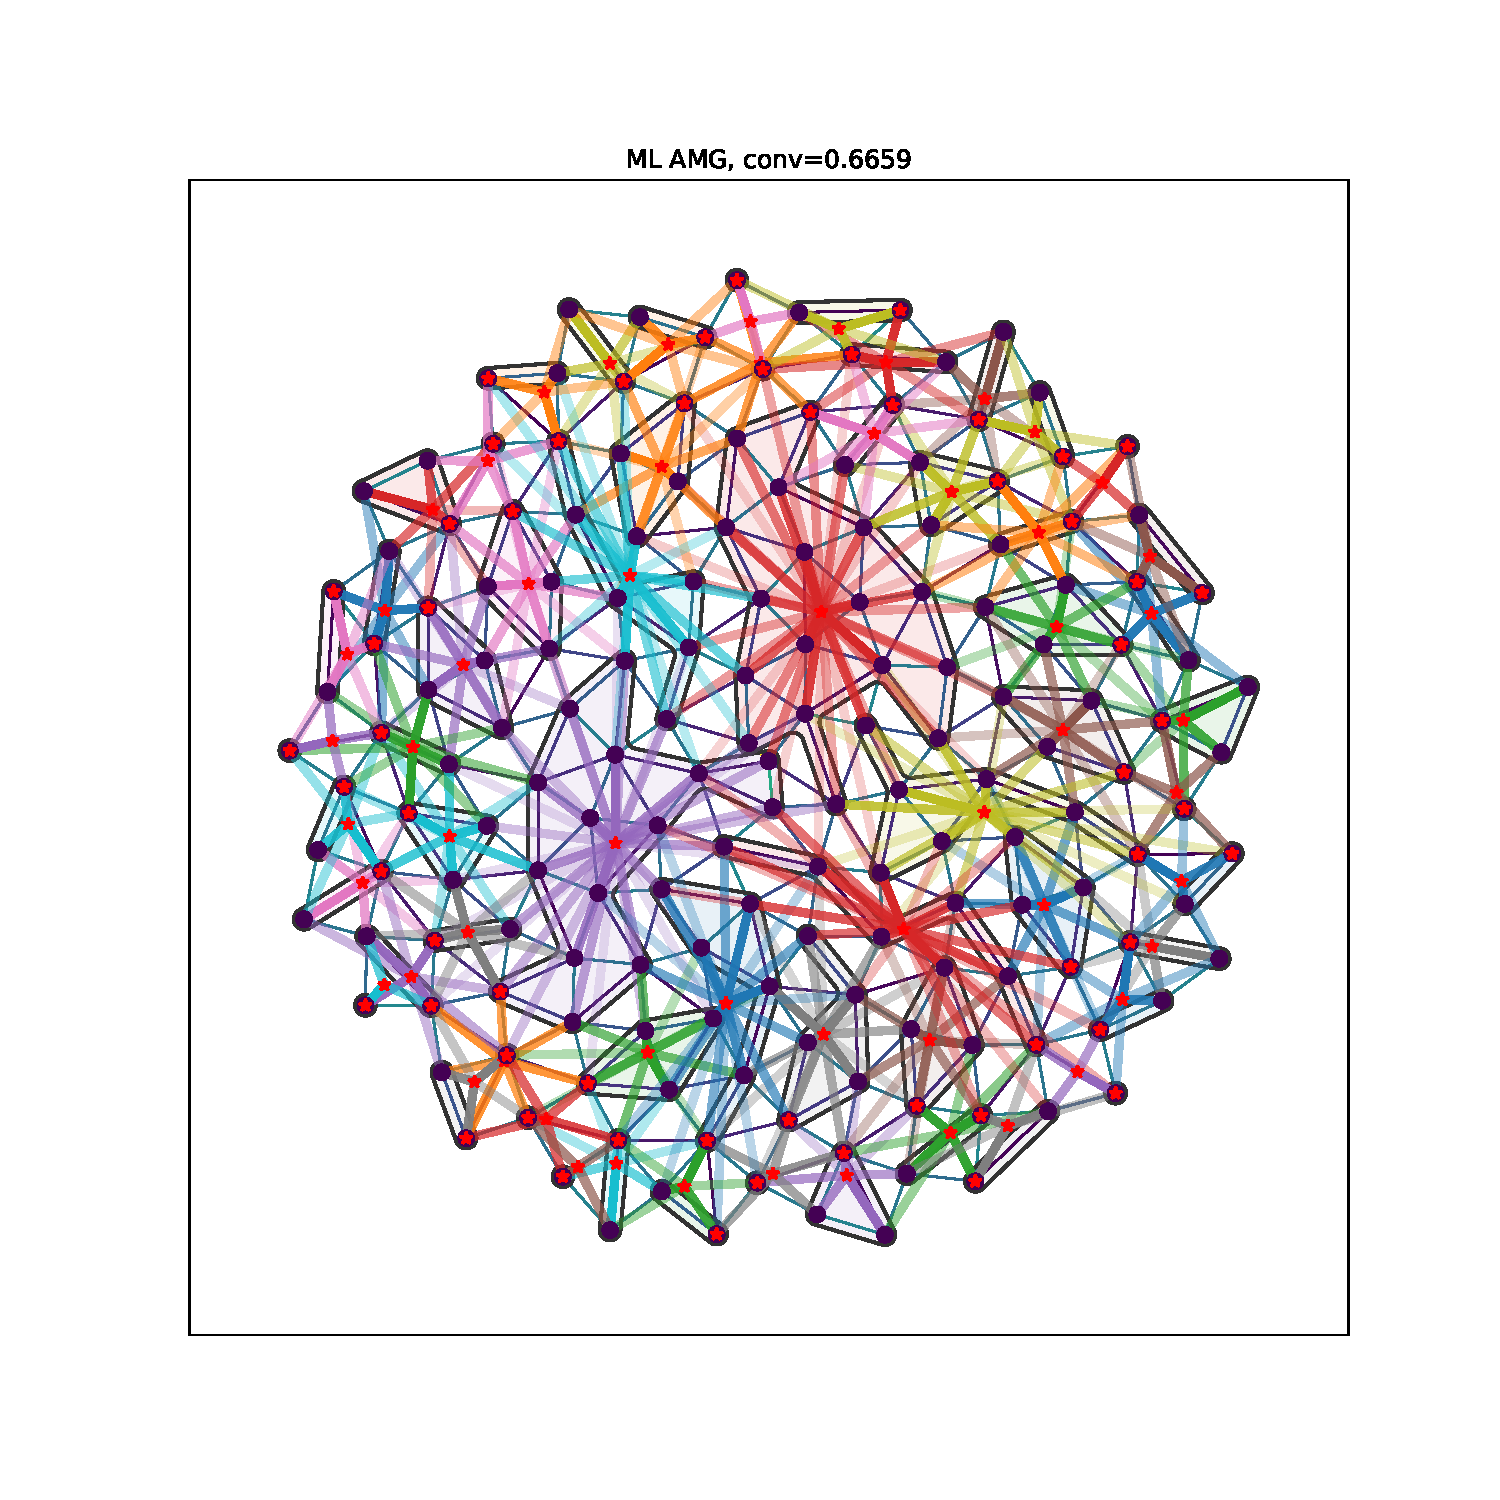
\includegraphics[width=\textwidth, trim=80 70 70 50, clip]{grid_circle_new.pdf}
    \caption{New ML}
  \end{subfigure}
  \caption{Aggregate and interpolation data for a circular unstructured mesh.  This particular mesh has 173 DoF.}
  \label{fig:gridcircle}
\end{figure}

\begin{figure}[h]
  \centering
  \begin{subfigure}[t]{0.32\textwidth}
    \centering
    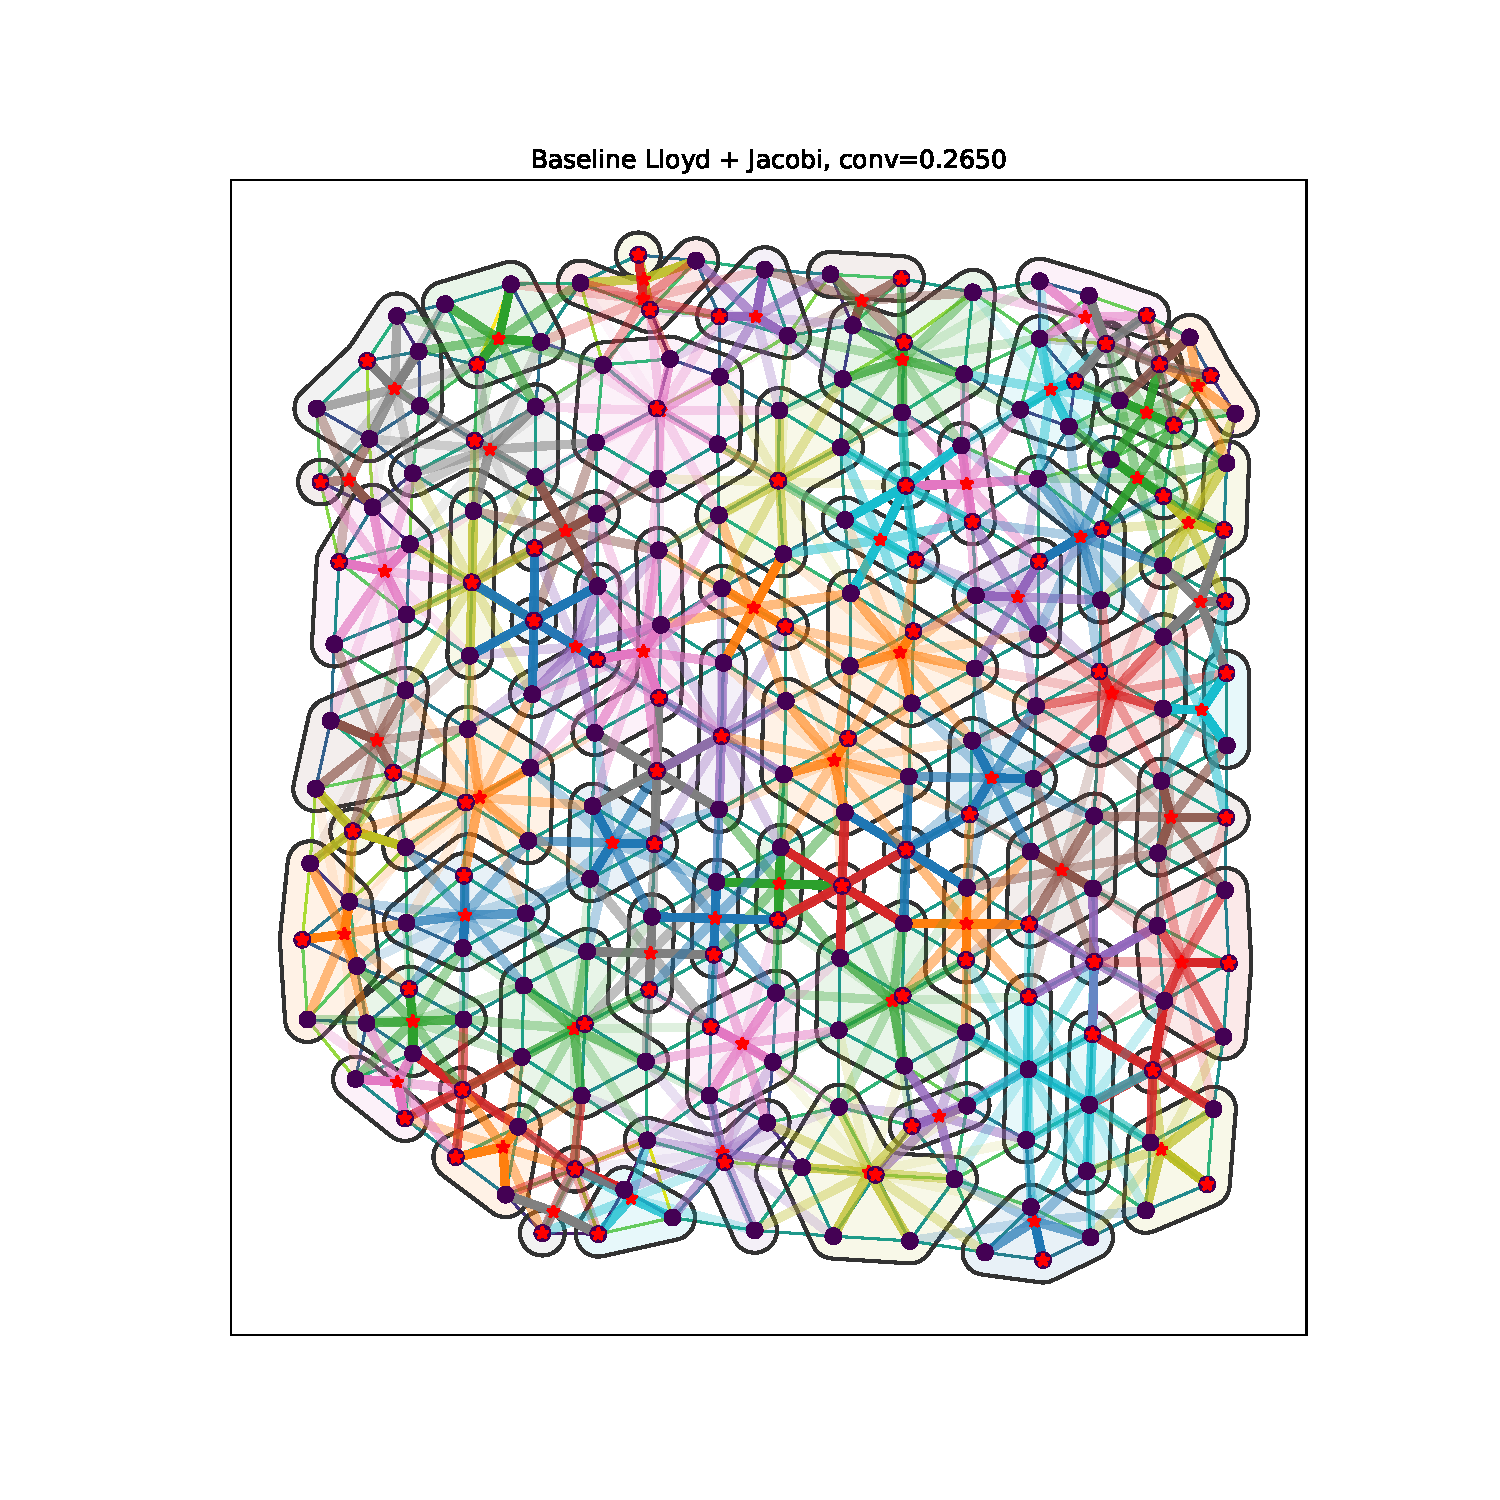
\includegraphics[width=\textwidth, trim=80 70 70 50, clip]{grid_700_lloyd.pdf}
    \caption{Lloyd + Jacobi}
  \end{subfigure}
  \begin{subfigure}[t]{0.32\textwidth}
    \centering
    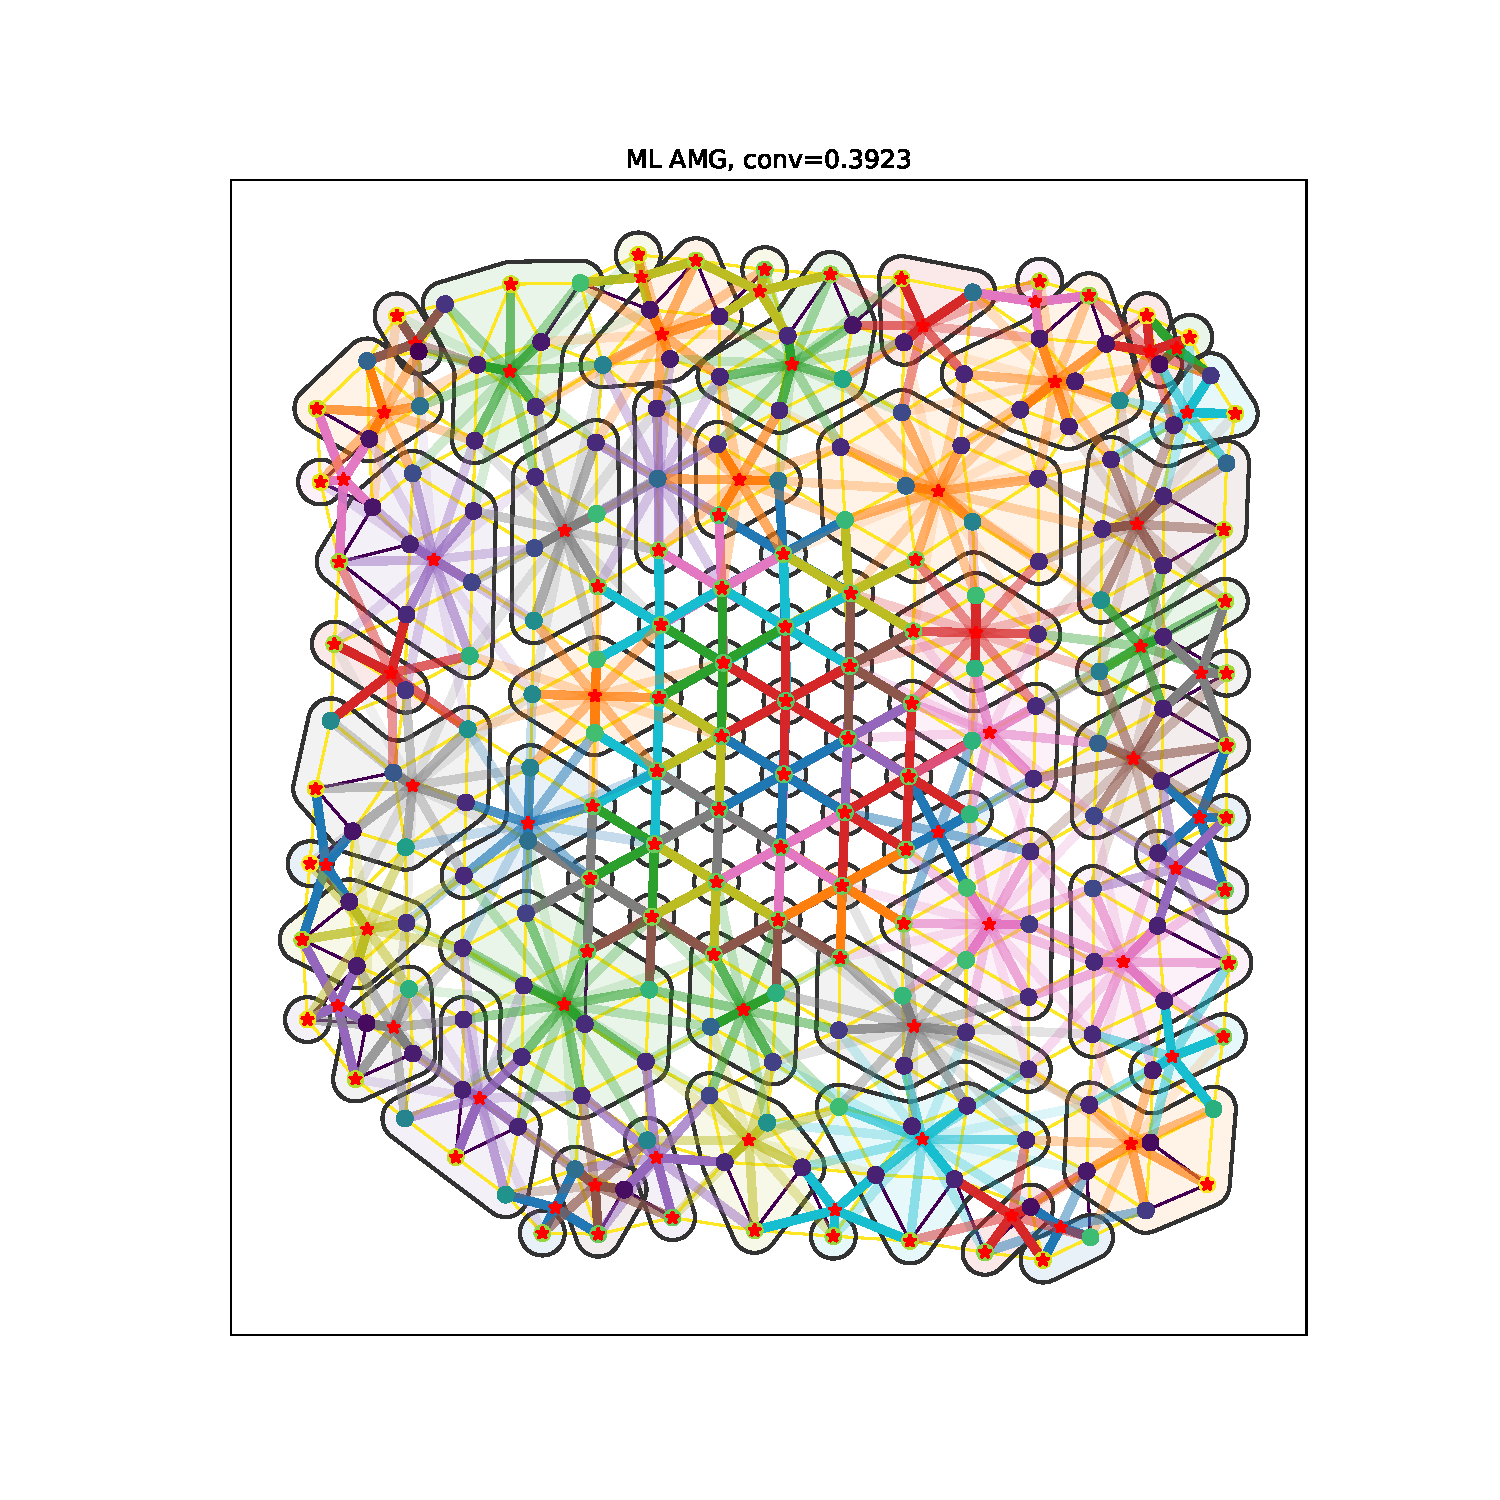
\includegraphics[width=\textwidth, trim=80 70 70 50, clip]{grid_700_ml.pdf}
    \caption{Old ML (Last Week)}
  \end{subfigure}
  \begin{subfigure}[t]{0.32\textwidth}
    \centering
    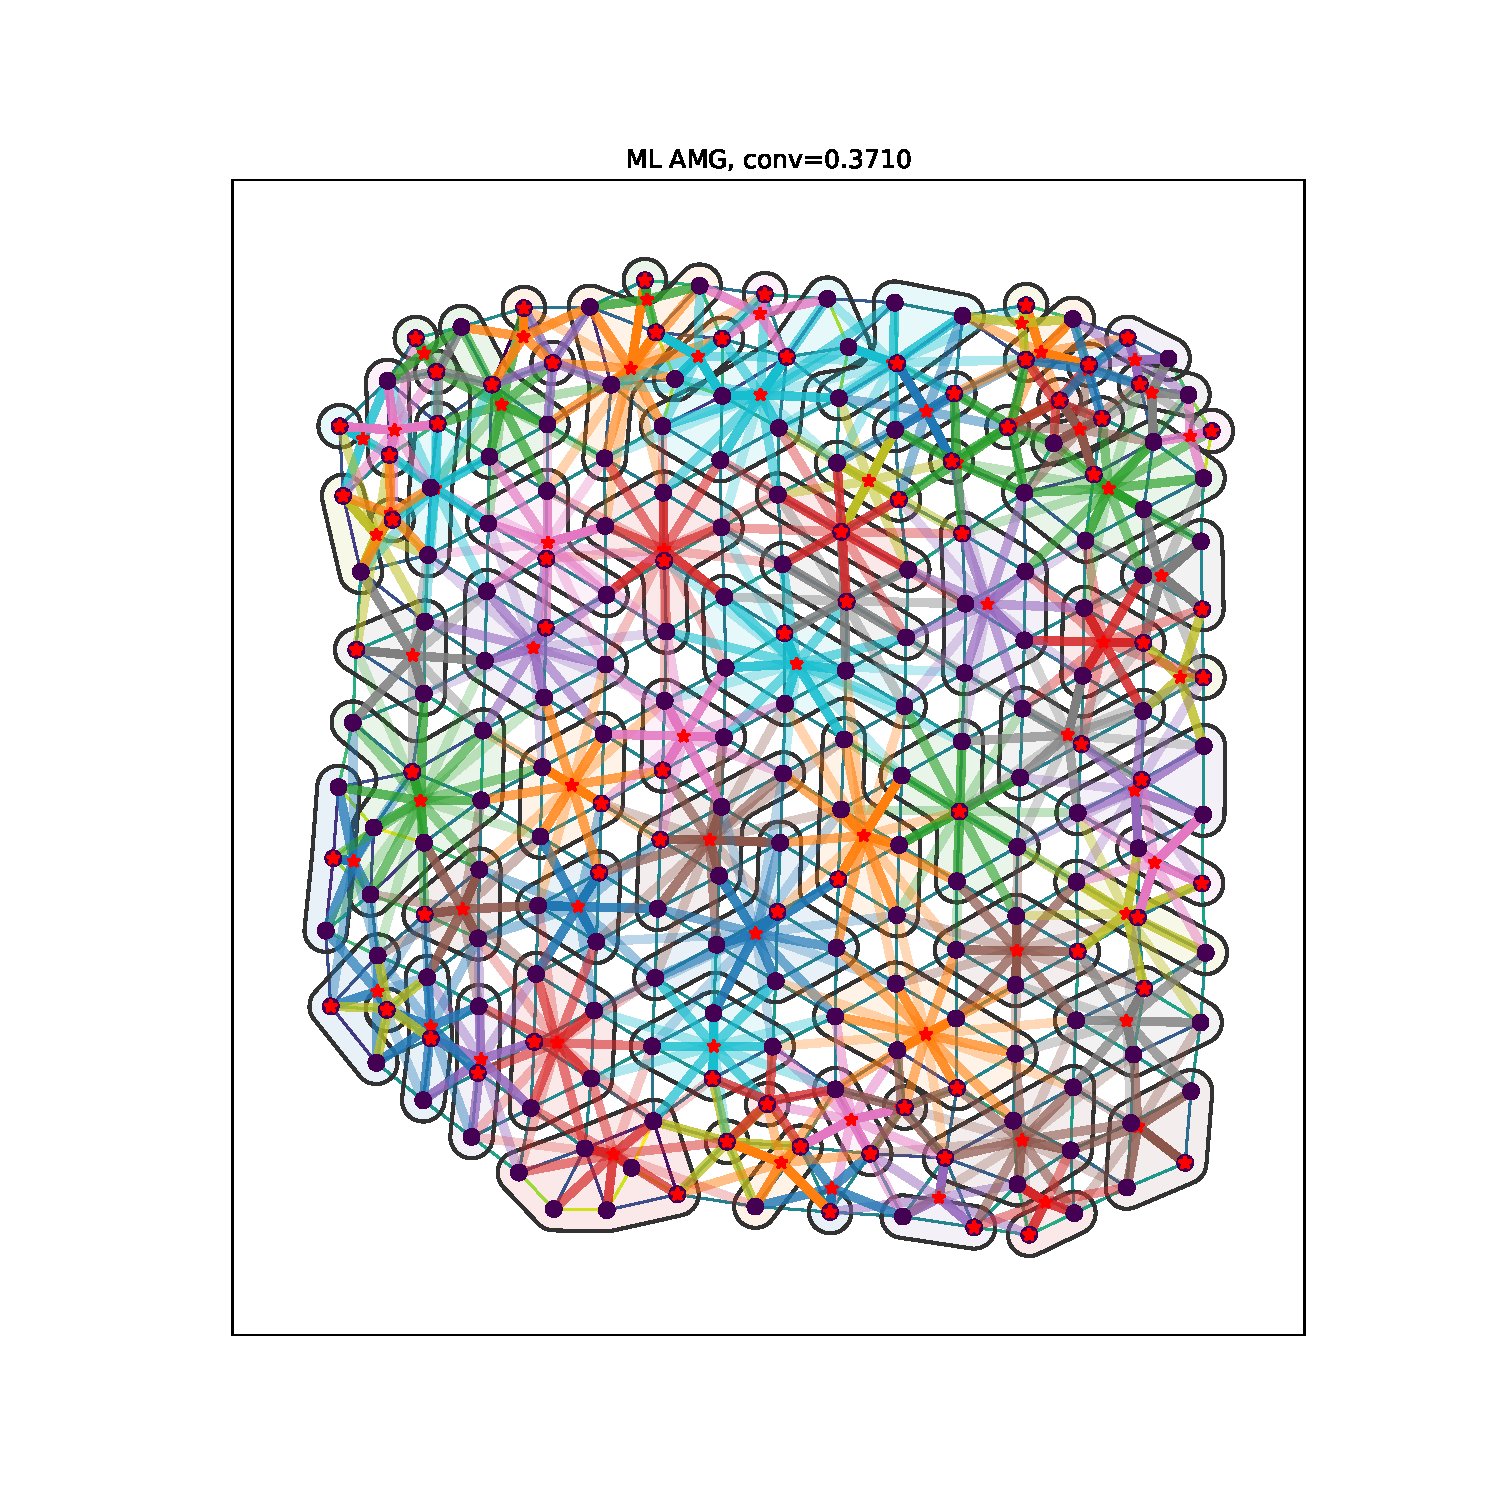
\includegraphics[width=\textwidth, trim=80 70 70 50, clip]{grid_700_new.pdf}
    \caption{New ML}
  \end{subfigure}
  \caption{Aggregate and interpolation data for a random unstructured mesh.  This particular mesh has 220 DoF.}
  \label{fig:grid700}
\end{figure}

\begin{figure}[h]
  \centering
  \begin{subfigure}[t]{0.32\textwidth}
    \centering
    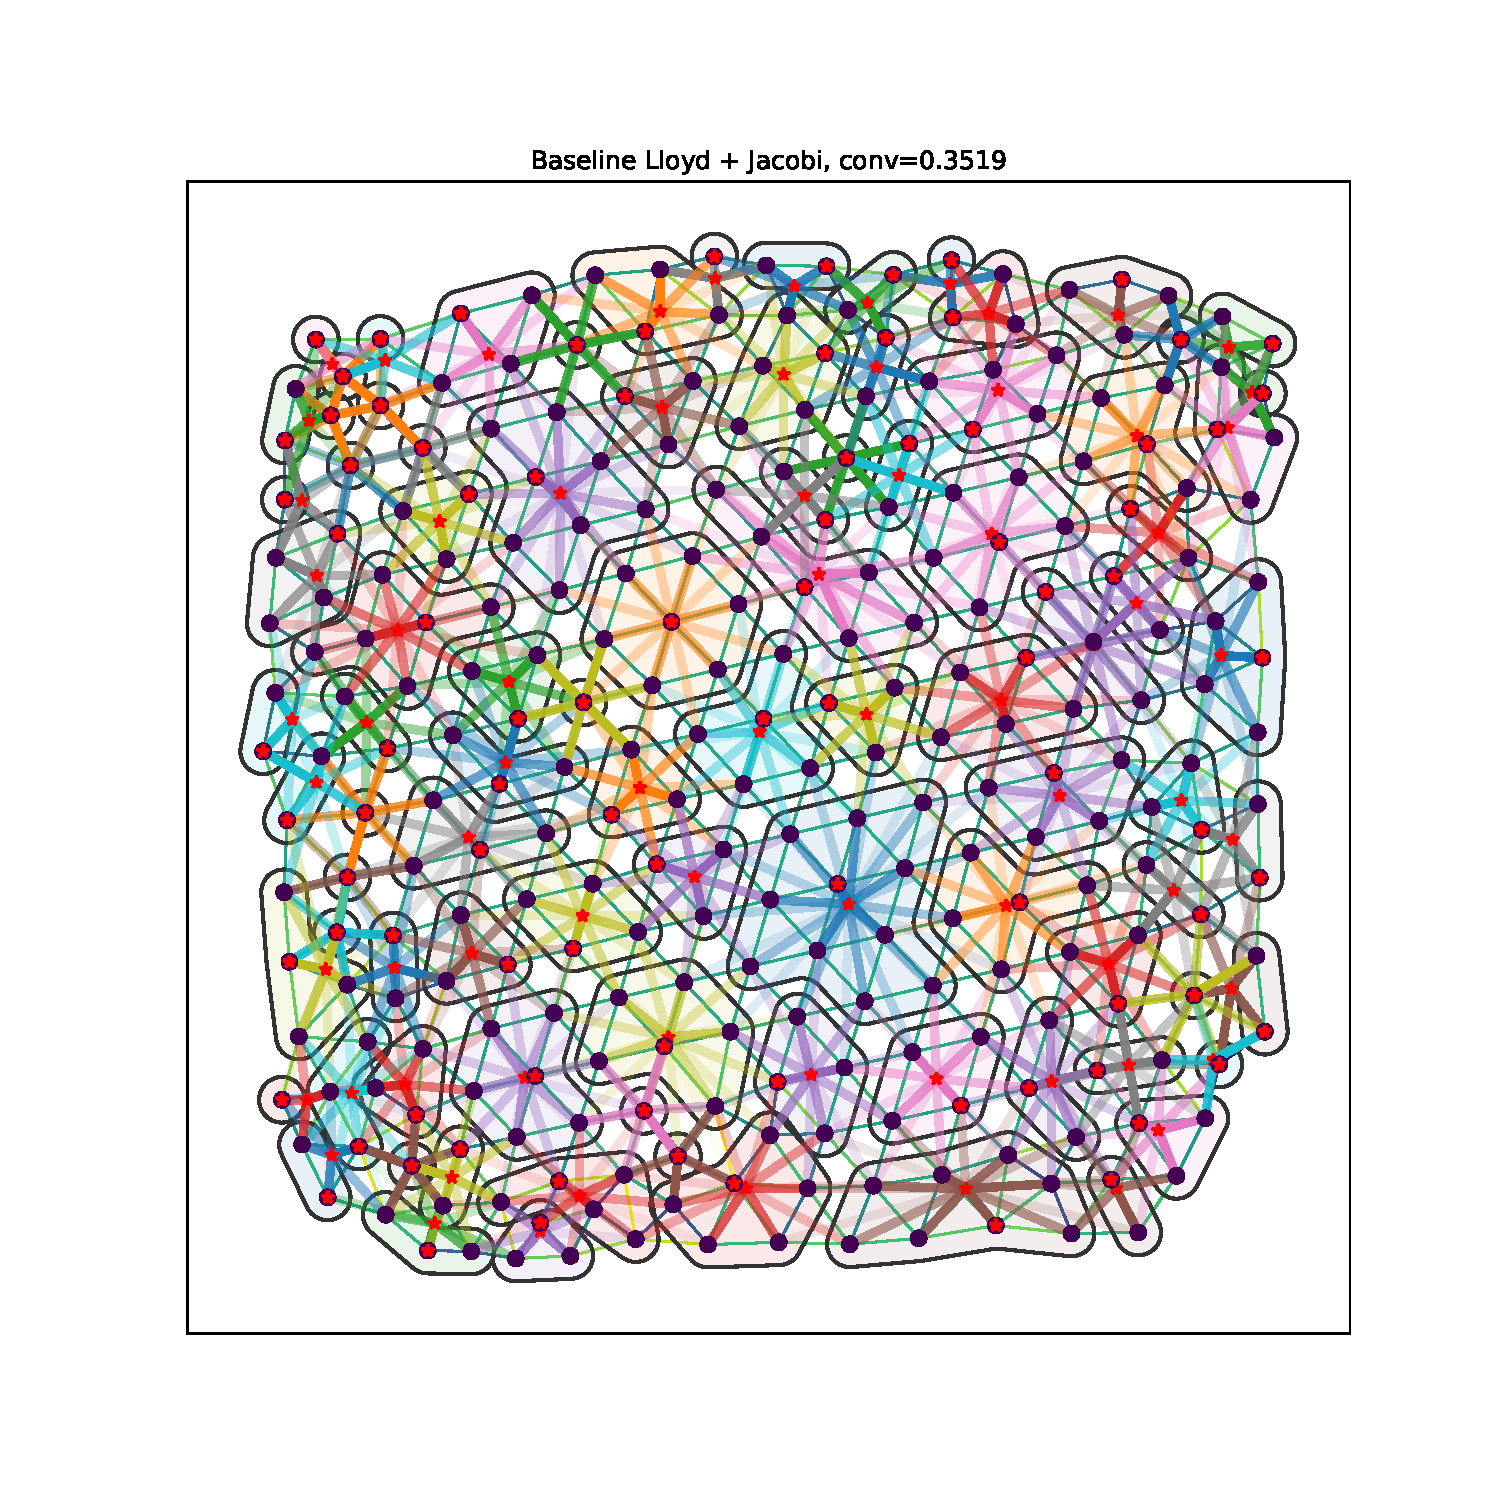
\includegraphics[width=\textwidth, trim=80 70 70 50, clip]{grid_800_lloyd.pdf}
    \caption{Lloyd + Jacobi}
  \end{subfigure}
  \begin{subfigure}[t]{0.32\textwidth}
    \centering
    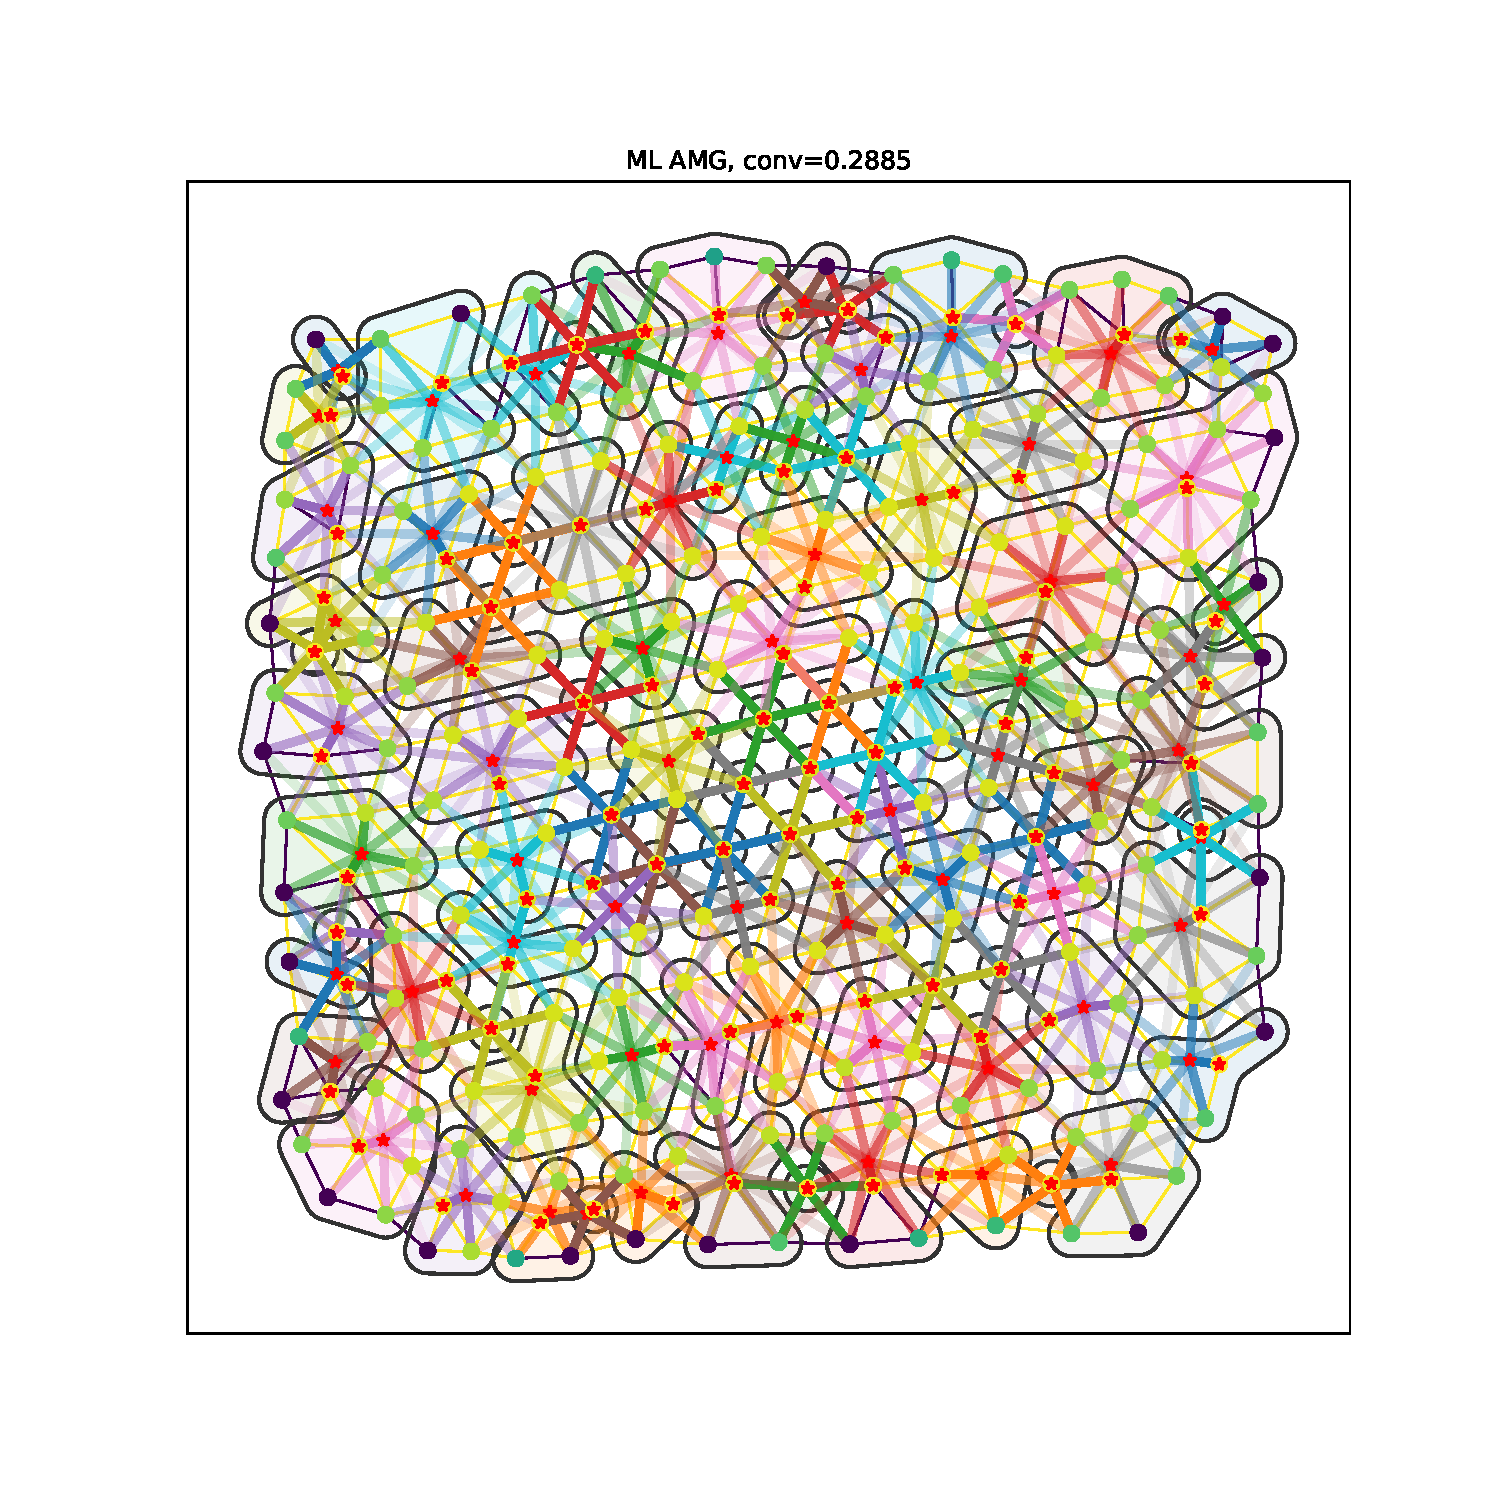
\includegraphics[width=\textwidth, trim=80 70 70 50, clip]{grid_800_ml.pdf}
    \caption{Old ML (Last Week)}
  \end{subfigure}
  \begin{subfigure}[t]{0.32\textwidth}
    \centering
    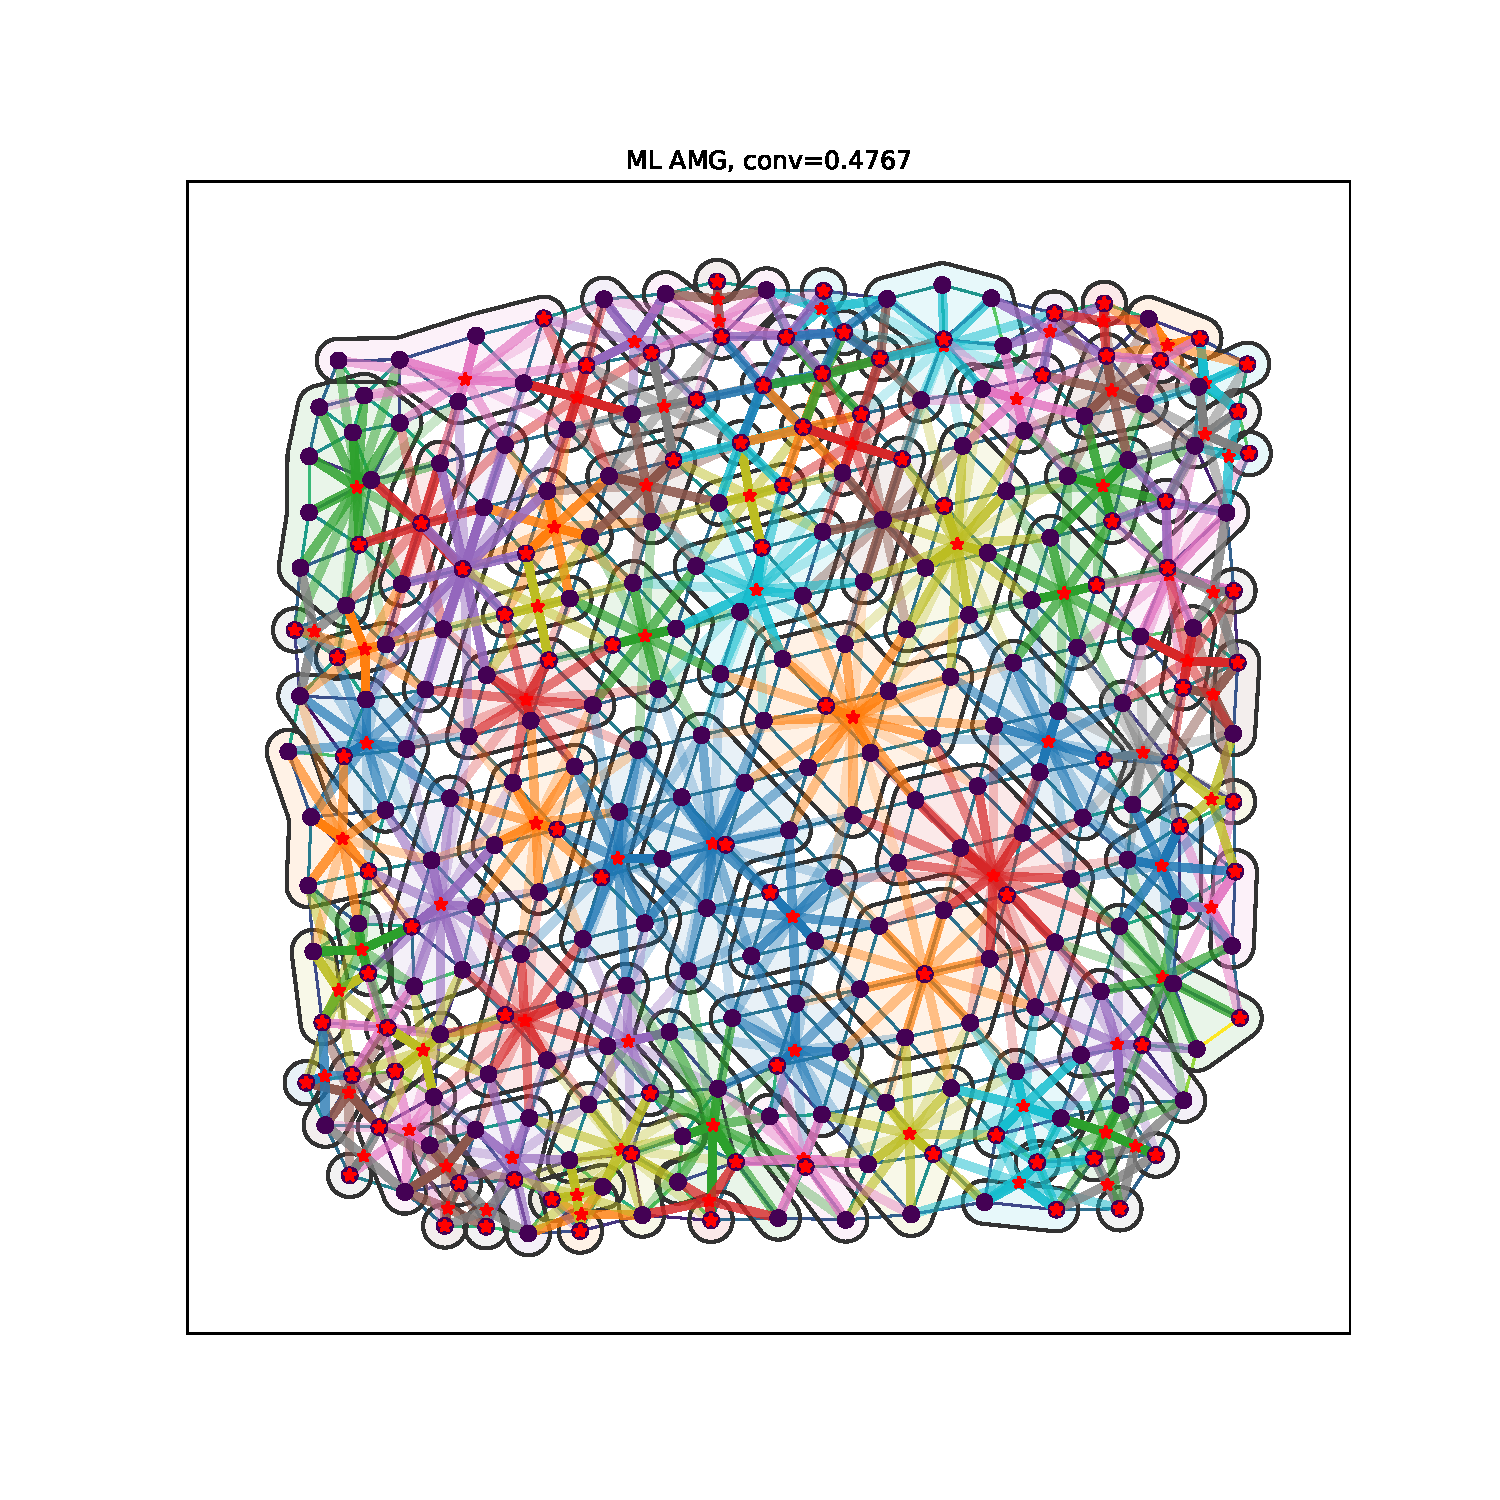
\includegraphics[width=\textwidth, trim=80 70 70 50, clip]{grid_800_new.pdf}
    \caption{New ML}
  \end{subfigure}
  \caption{Aggregate and interpolation data for a random unstructured mesh.  This particular mesh has 273 DoF.}
  \label{fig:grid800}
\end{figure}

\begin{figure}[h]
  \centering
  \begin{subfigure}[t]{0.32\textwidth}
    \centering
    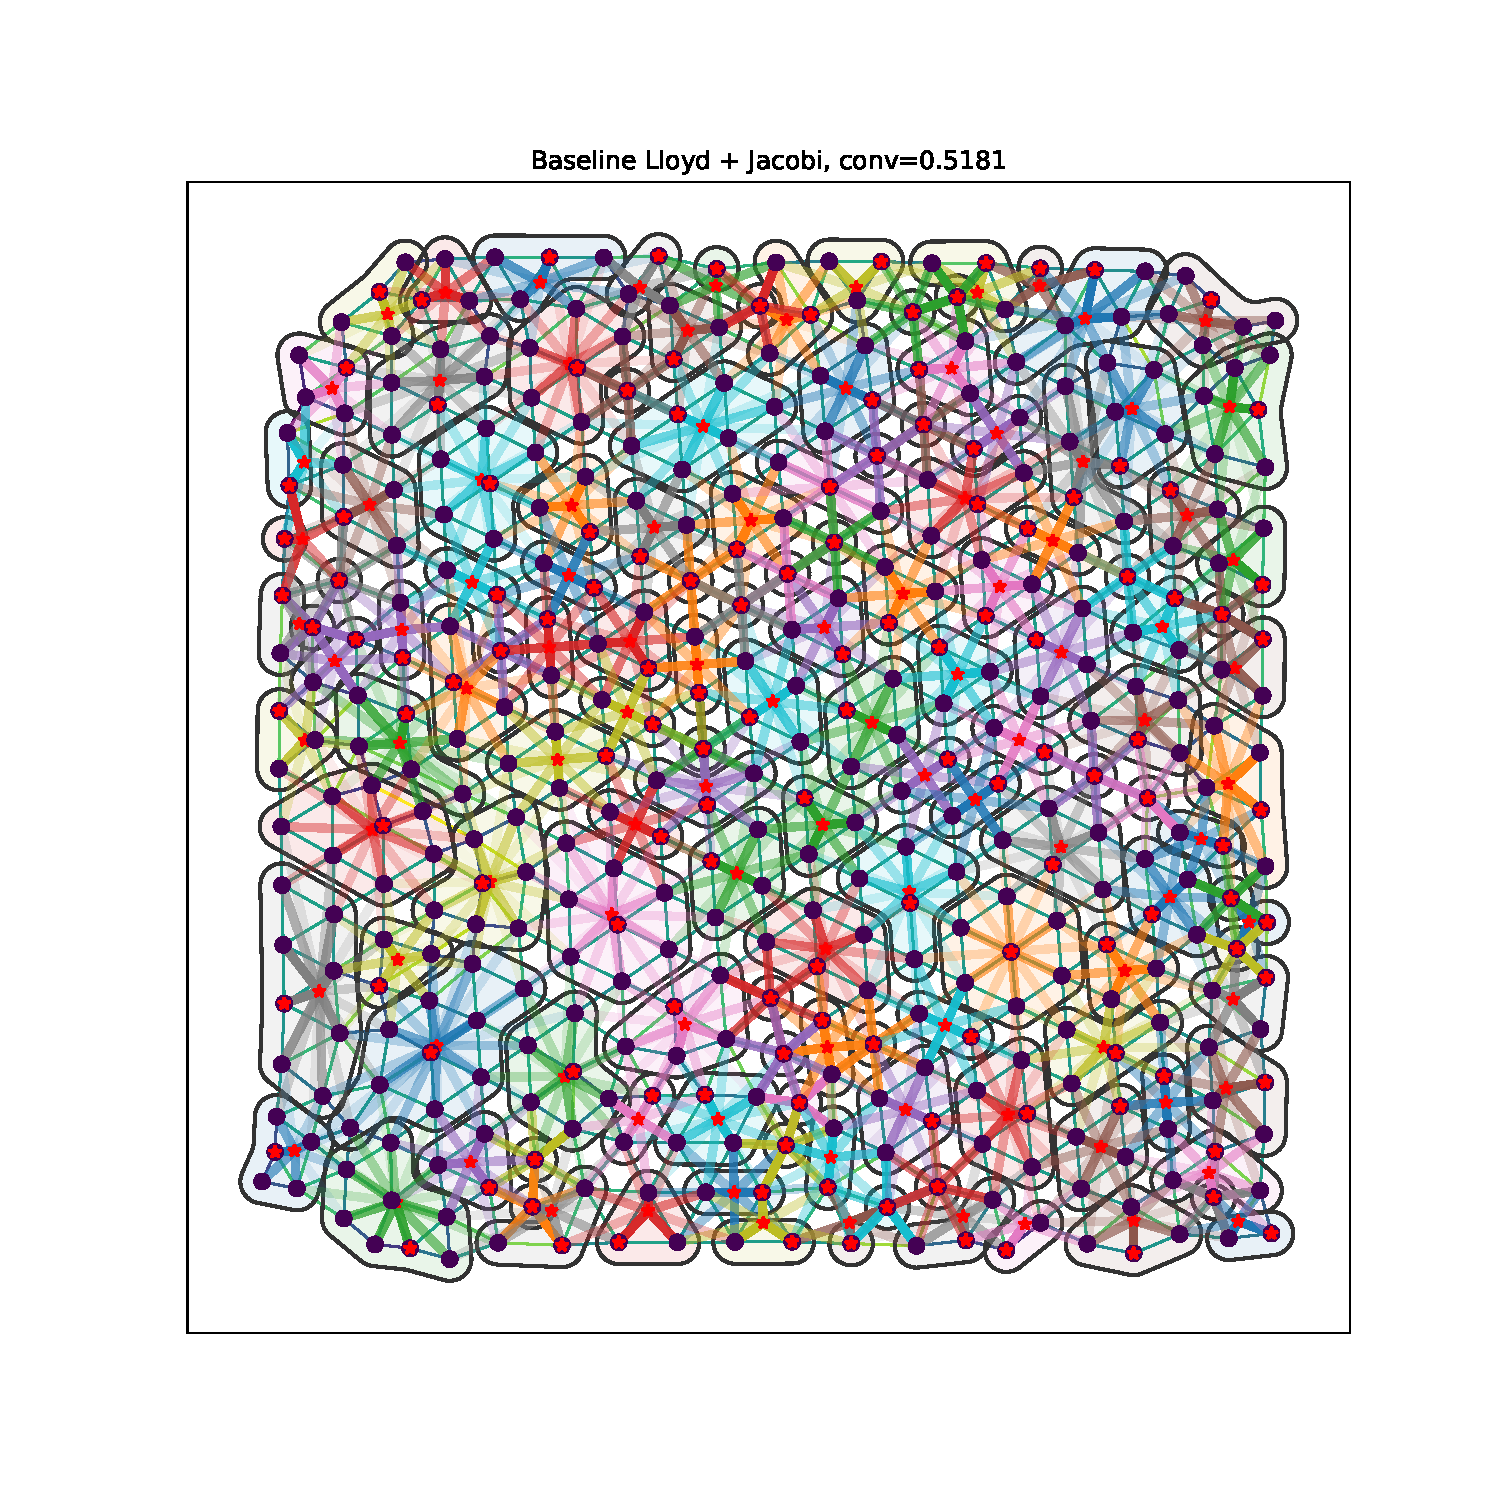
\includegraphics[width=\textwidth, trim=80 70 70 50, clip]{grid_largest_lloyd.pdf}
    \caption{Lloyd + Jacobi}
  \end{subfigure}
  \begin{subfigure}[t]{0.32\textwidth}
    \centering
    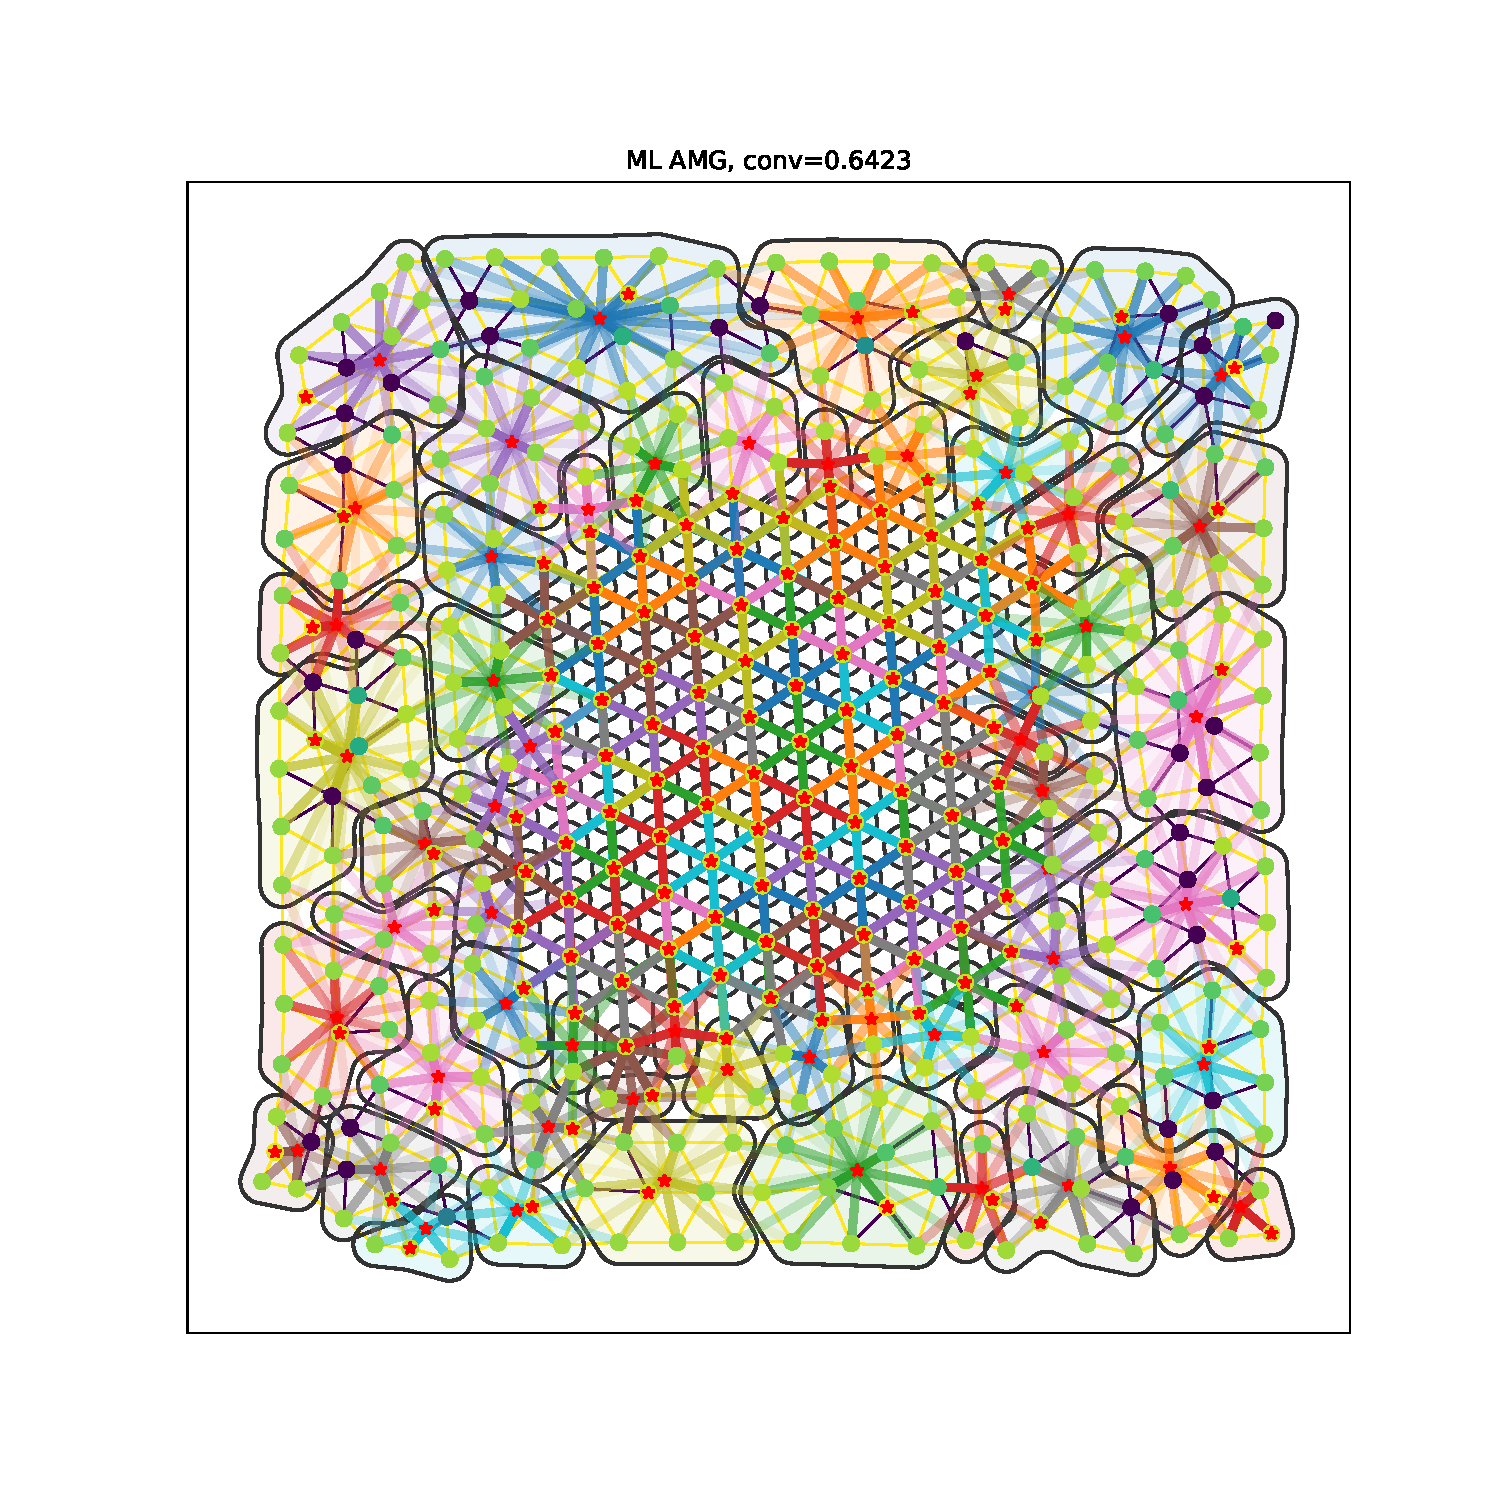
\includegraphics[width=\textwidth, trim=80 70 70 50, clip]{grid_largest_ml.pdf}
    \caption{Old ML (Last Week)}
  \end{subfigure}
  \begin{subfigure}[t]{0.32\textwidth}
    \centering
    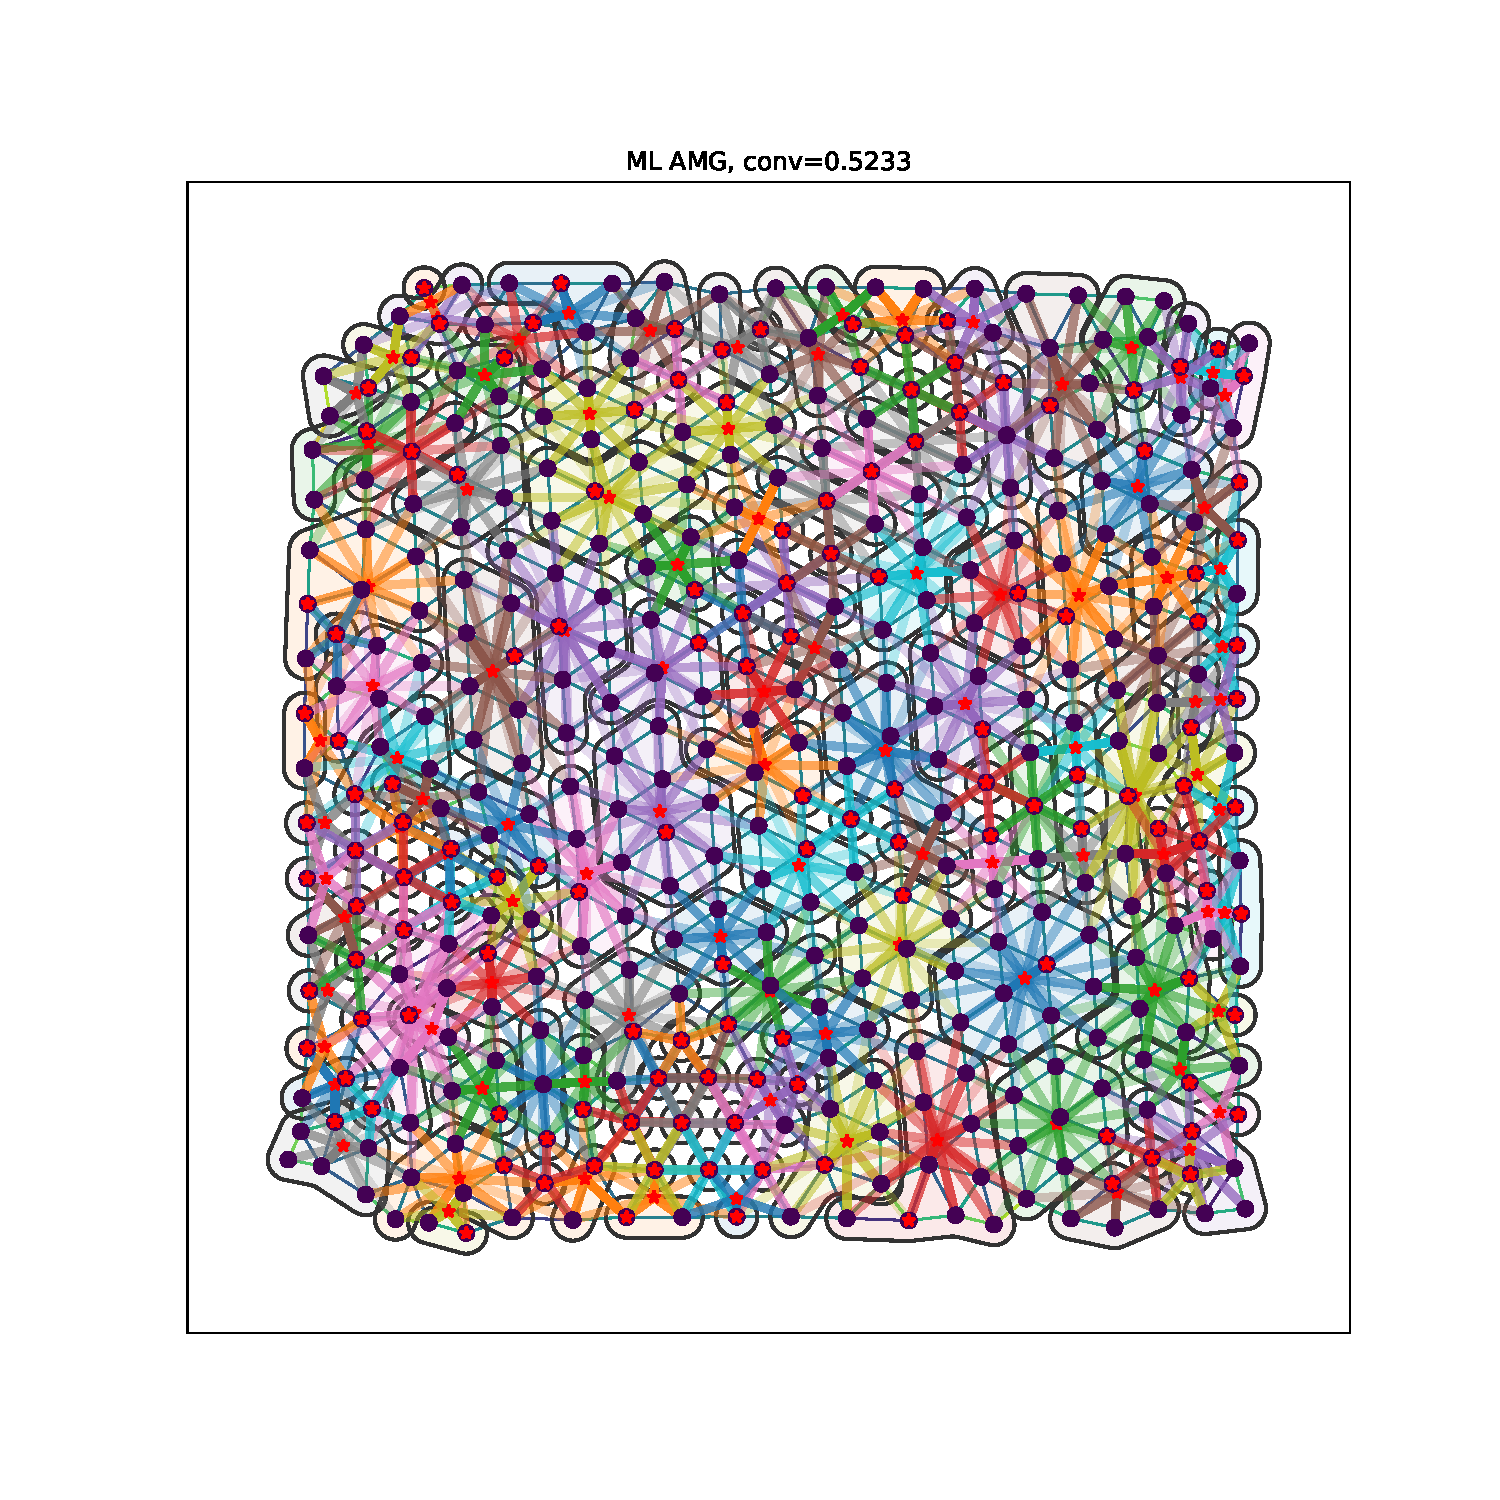
\includegraphics[width=\textwidth, trim=80 70 70 50, clip]{grid_largest_new.pdf}
    \caption{New ML}
  \end{subfigure}
  \caption{Aggregate and interpolation data for the largest mesh in the \textit{training set}.  This particular mesh has 410 DoF.}
  \label{fig:grid800}
\end{figure}

%% \section{Discussion}
%% Currently the loss is computed as
%% \begin{equation}
%%   \ell := \frac{1}{n} \sum_i^n c_{\text{ML}}\left(i\right),
%% \end{equation}
%% where $c_{\text{ML}}\left(i\right)$ is the ML convergence of the $i$'th problem.  Perhaps it be worth computing the loss as instead
%% \begin{equation}
%%   \ell := \frac{1}{n} \sum_i^n \frac{c_{\text{ML}}\left(i\right)}{c_{\text{Lloyd}}\left(i\right)},
%% \end{equation}
%% where each problem is instead normalized by the baseline performance.  Each term inside the summation can be thought of as the \textit{relative performance} of the ML method versus Lloyd, with $c<1$ indicating a lower convergence and $c>1$ indicating higher performance.

\bibliographystyle{siam}
\bibliography{navier}
\end{document}
